\chapter{Measurements and OGS Observation Links}
\label{chap:measurements}

\definecolor{gqQuestionBg}{gray}{0.93}
\definecolor{gqReady}{HTML}{1B7F3A}
\definecolor{gqDiagnostic}{HTML}{087F8C}
\definecolor{gqPolicy}{HTML}{6F42C1}
\definecolor{gqGate}{HTML}{D97706}
\definecolor{gqBlocked}{HTML}{B42318}
\newcommand{\gqStatus}[2]{\textcolor{#1}{\textbf{#2}}}
\newcommand{\gqPair}[4]{%
  \rowcolor{gqQuestionBg}%
  \multicolumn{2}{@{}L{0.94\textwidth}@{}}{\textbf{Question.} #3}\\*%
  \textbf{Answer.} & #4\\%
  \addlinespace[0.42em]%
}
\newcommand{\gqGroundingTable}[3]{%
  \Needspace{14\baselineskip}%
  \begin{center}%
  \footnotesize%
  \renewcommand{\arraystretch}{1.16}%
  \setlength{\tabcolsep}{4pt}%
  \captionof{table}{#2}%
  \label{#1}%
  \begin{tabular}{@{}L{0.17\textwidth} L{0.77\textwidth}@{}}%
  \toprule%
  #3%
  \bottomrule%
  \end{tabular}%
  \end{center}%
}

\section{Purpose and Evidence Boundary}
\label{sec:measurement-purpose}

This chapter records the measurement side of the CD-A Niche 4 modelling problem.
The purpose is not to turn every available dataset into a likelihood term.  The
purpose is to state, stream by stream, what is measured, where and when it is
measured, which unit and reference convention are used, and how the value can enter
the OGS workflow as an input, output residual, material-field prior, diagnostic, or
caveat.
\revreplaceonly{9}{OGS tie}{model link}{\annCommentNine}
\revadd{31}{This is why each measurement stream first states the measured quantity
and support before assigning any model link, residual role, diagnostic role, or
gate.}{\pdfAnnComment{14}{Obecne je treba vysjasnit, co presne meri ktery
experiment. Tohle je k vyjasneni prakticky ke kazde otazce tohoto seznamu.}{The
chapter structure now answers this globally: every stream defines what is measured
before it states the OGS observation role.}}

The primary evidence for the plotted data and row summaries is the set of
email- and TeamBeam-provided source files named in the bibliography.  We use the
processed observation tables and generated measurement figures copied into this
paper as traceable reductions of those files.  The processed-observation layer is
the authority for row counts, time ranges, coordinate status, and current activation
gates \citep[source filenames and transfer context]{CDAProvidedMeasurementFiles2025}.
Public internet sources were checked only where the provided source catalogue lacks
residual-ready numeric exports.  They confirm the broader CD/CD-A monitoring
context, including pressure, extensometer, crackmeter, Taupe/TDR, RH, water-content,
and resistivity streams, but they do not replace the missing project-specific
Geoscope, pressure, or crack-opening time series
\citep[abstract and Sec.~2]{Ziefle2017SeasonalHM}
\citep[Secs.~2.4 and 3.2]{Graebling2022VEIS}.

The geometry rule is the same for all streams.  A measurement is not an OGS datum
until its support is mapped into the current two-dimensional model frame.  Point
measurements need coordinates and a sampling rule.  Borehole interval measurements
need segment geometry and interval weights.  ERT needs a mesh-to-mesh observation
operator.  Taupe/TDR needs line-band support.  HM monitoring needs a reference
frame, instrument sign convention, and a 3D-to-2D reduction policy before it can be
weighted.

The model-facing scope in this report is the open-niche side.  In the provided
source-layout geometry the open twin is the negative-\(x\) niche
\path{Open_twin}; after the processed OGS/ERT projection this side is the
near-origin cluster and the ERT loop.  The measurement-coordinate rows around
\(x\approx 12\)--\(19\,\mathrm{m}\) are the opposite/closed-side context and are
not part of the current open-niche comparison unless a section explicitly marks
them as qualitative source context
\citep[source filenames and support reductions]{CDAProvidedMeasurementFiles2025}.

\begin{figure}[htbp]
  \centering
  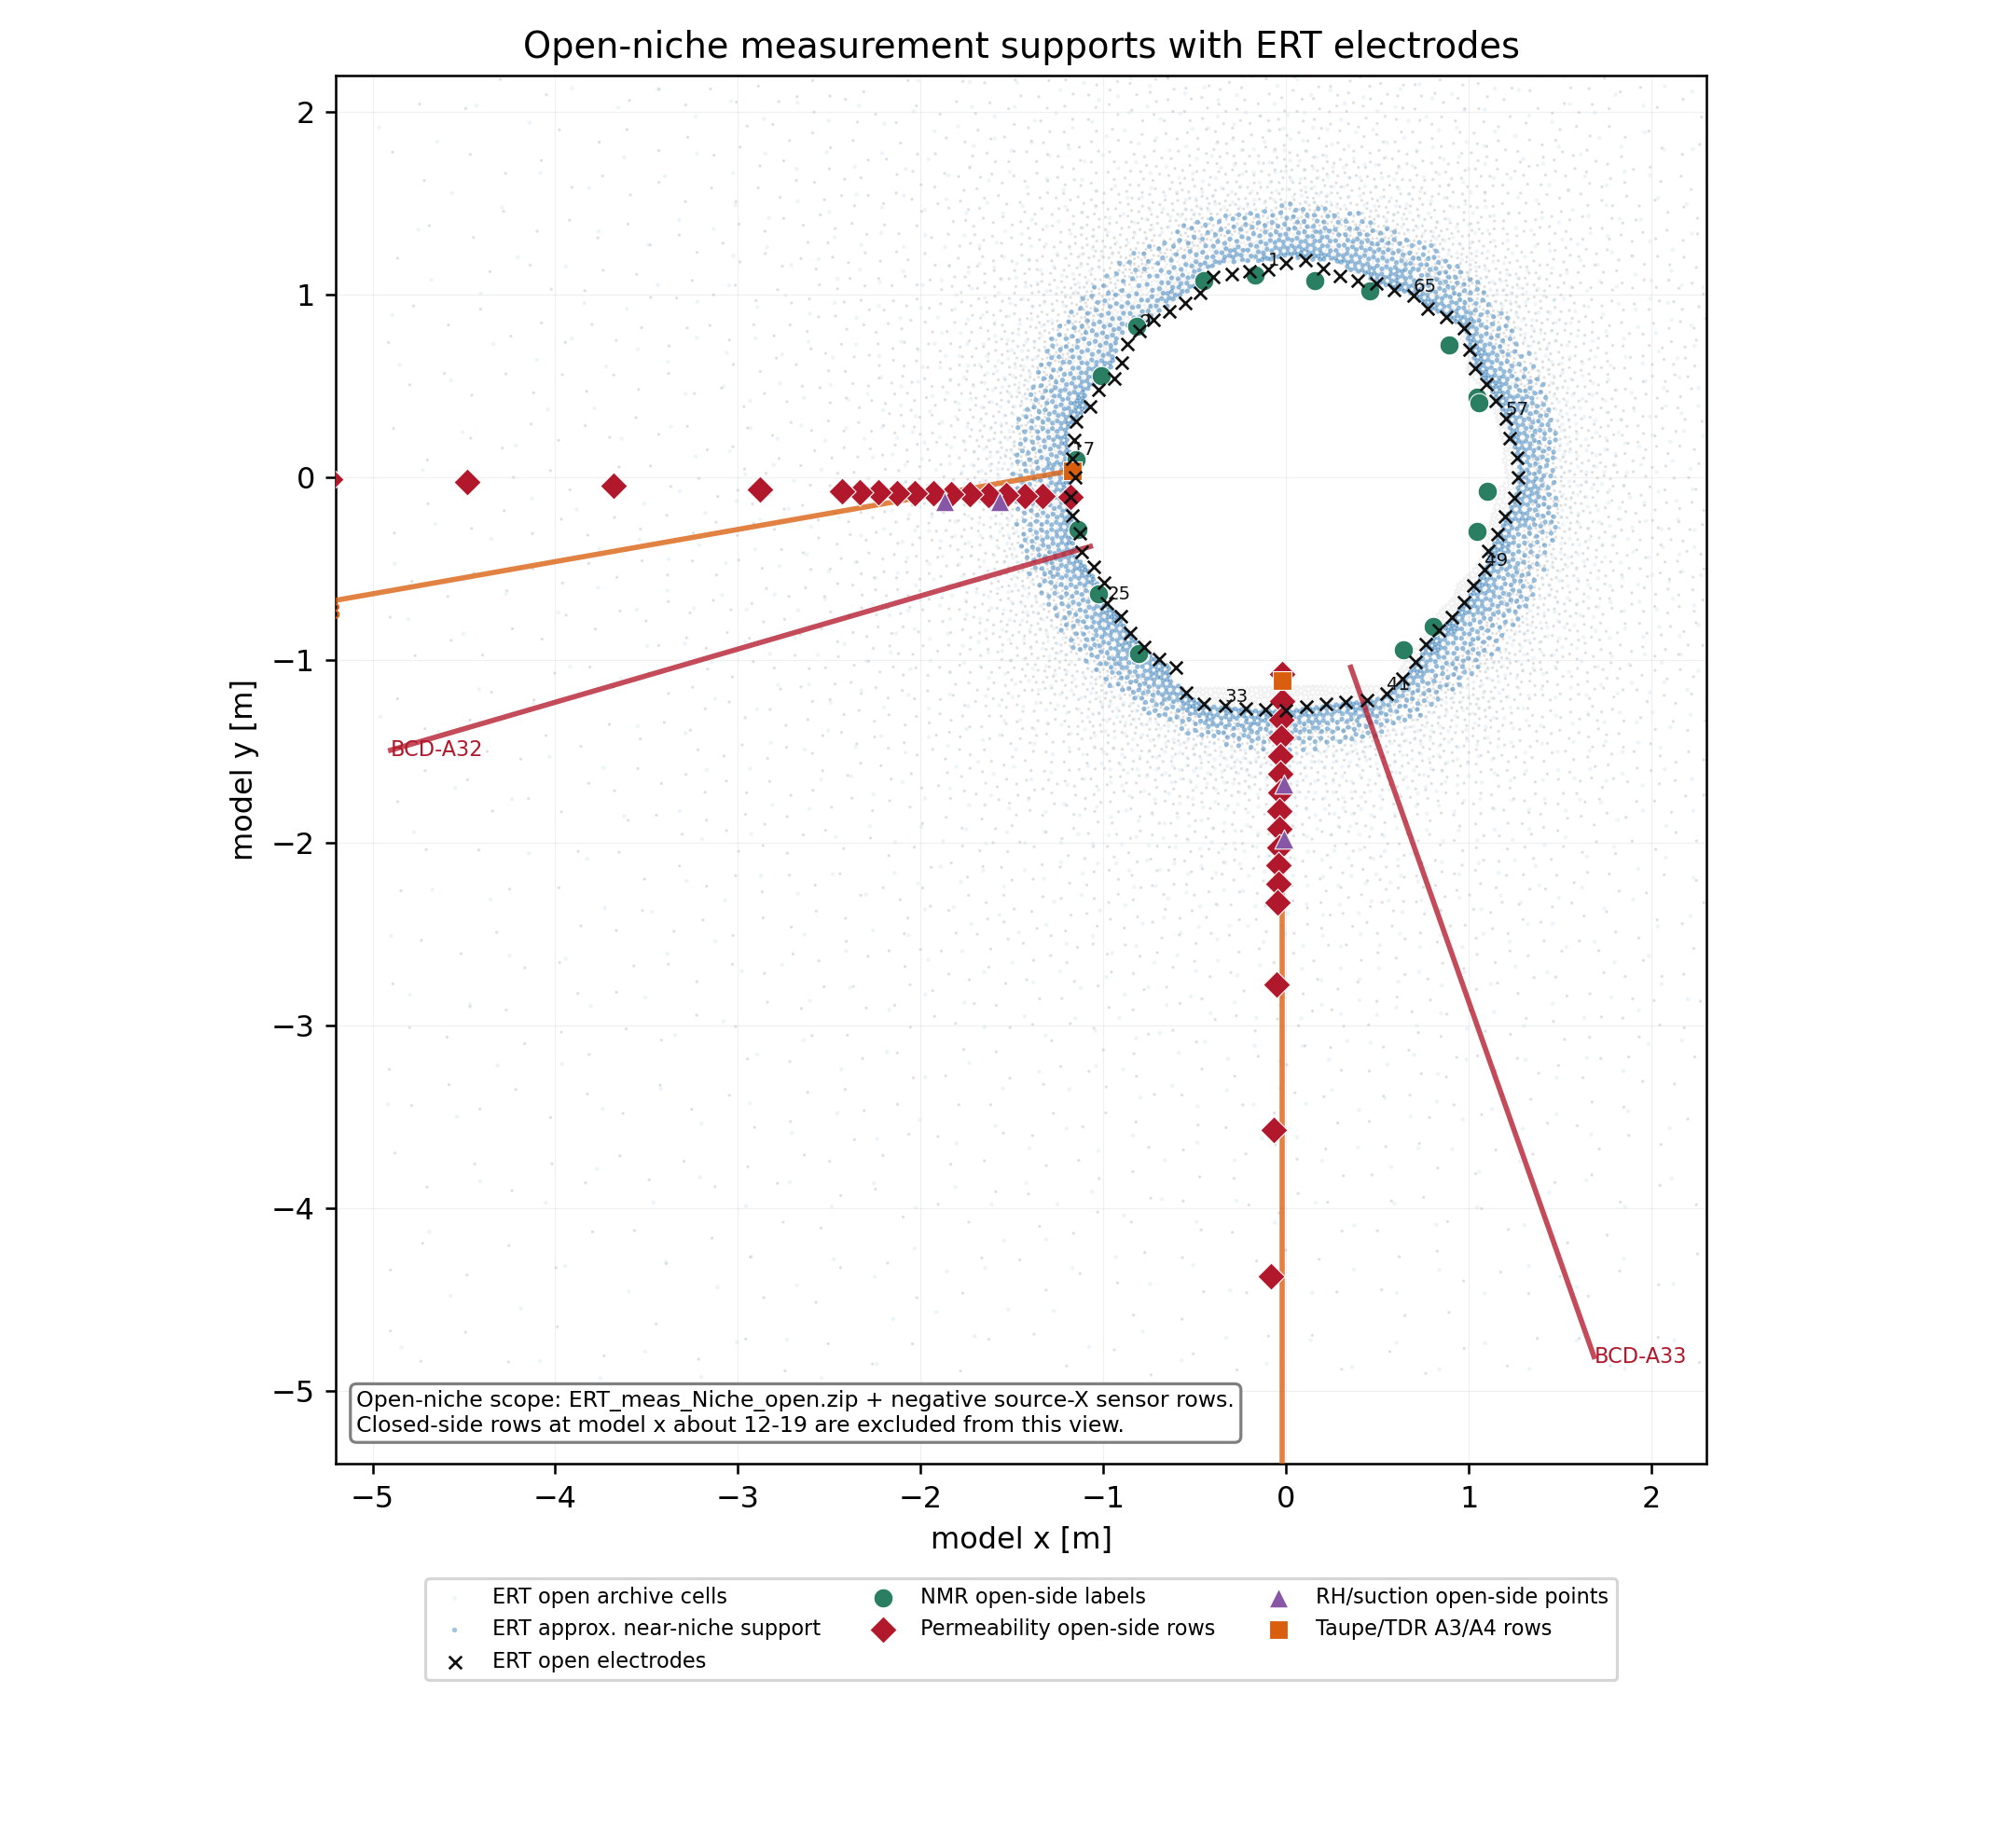
\includegraphics[width=0.90\textwidth]{resources/figures/measurement_locations_open_niche_ert.png}
  \caption{Open-niche measurement supports in the current OGS domain.  The plot
  shows the open ERT electrode loop, projected ERT support cells, NMR labels,
  Taupe/TDR A3/A4 supports, RH/suction points, and open-side permeability
  pulse-test intervals.  Closed-side rows at \(x\approx 12\)--\(19\,\mathrm{m}\)
  are excluded from the current model-facing scope.}
  \label{fig:measurement-locations-all}
\end{figure}

\begin{longtable}{@{}L{0.19\textwidth} L{0.19\textwidth} L{0.23\textwidth} L{0.30\textwidth}@{}}
\caption{Measurement stream roles in the current OGS workflow.}
\label{tab:measurement-role-summary}\\
\toprule
Stream & Current status & Model link & Main gate or use\\
\midrule
\endfirsthead
\caption[]{Measurement stream roles in the current OGS workflow (continued).}\\
\toprule
Stream & Current status & Model link & Main gate or use\\
\midrule
\endhead
\bottomrule
\endlastfoot
Permeability pulse tests &
Active material likelihood &
Direct interval-scale observation of intrinsic permeability \(\KK(\xx)\). &
Usable for 75 mapped open-twin BCD-A32/A33 rows; support conflicts and older
endpoint geometry remain gates.\\
NMR water content &
Active but provisional state likelihood &
Observation of water-content state, compared to \(\theta=\por\Sl\) after an
observation policy. &
Niche 4/open-side rows are relevant here; raw absolute water content is caveated by
bound/interlayer water; trend/anomaly is the preferred next residual.\\
ERT &
Diagnostic state field &
Forward operator from \(\Sl\) to water content to bulk resistivity to projected ERT
resistivity. &
The source archive and electrode loop used here are the open-niche ERT files; the
transform, support mask, and covariance remain gates before likelihood use.\\
Taupe/TDR &
Diagnostic trend field &
EDZ-band trend operator tied to \(\theta=\por\Sl\), or to dielectric/water-content
calibration if confirmed. &
Absolute unit and calibration are not confirmed; A3/A4 are the open-side supports,
while A7/A8 remain closed-side source context.\\
RH/suction &
Boundary-condition check &
Kelvin conversion to pressure or suction candidate for the open-niche boundary
\(p_E(t)\). &
Active curve provenance, filtering, time origin, and uncertainty remain open.\\
Direct pressure sensors &
Blocked future pressure residual &
Candidate samples of \(\pl(\xx,t)\) or hydraulic head. &
Mini-piezometer numeric time series, units, reference convention, and quality flags
are missing.\\
Fault/fracture geometry &
Structural prior or scenario field &
Candidate prior for permeability, porosity, EDZ masks, or 2D projection scenarios. &
3D geometry, measured aperture/effect, timing, and projection policy are incomplete
for hard use.\\
Other HM monitoring &
Blocked or qualitative HM validation &
Candidate displacement, strain, crack opening, levelling, scan-difference, or
pressure residuals. &
Layout and levelling summaries exist; hard residuals need numeric exports,
timestamps, units, reference zeros, and uncertainties.\\
\end{longtable}

\revadd{2}{Uncertainty is stream-specific in the current evidence set.  Direct
permeability uses a conservative \(0.5\) log10-unit policy and
duplicate-aware weighting.  NMR has reported confidence intervals and a floor, but
absolute values remain biased by bound/interlayer water.  ERT, Taupe/TDR,
RH/suction, direct pressure, fracture geometry, and HM streams retain gates until
their covariance, calibration, support, and reference conventions are supplied.}{\annCommentTwo}
\revadd{2}{For practical weighting, only direct permeability and the ERT inversion
reports currently carry explicit numeric likelihood scales in this paper: direct
permeability uses the \(0.5\) log10-unit policy, and the ERT inversion reports use
log10-resistivity residual scales such as \(\sigma_\rho=0.18\).  The other streams
remain diagnostic or gated until their own noise model is supplied.}{\annCommentTwo}

\section{Direct Permeability Pulse Tests}
\label{sec:measurement-permeability}

\paragraph{Meaning.}
The permeability stream records interpreted pulse-test permeability values,
transmissibility values, and raw pressure-decay traces.  The source method is a
modified double-piston packer test with a nominal 10 cm interval and nitrogen
injection.  Therefore the model-facing quantity is a gas-test interpretation of
intrinsic permeability, not hydraulic conductivity, not liquid relative permeability,
and not a direct tensor component.  Gas apparent permeability has its own pressure
dependence, so the liquid-equivalent intrinsic value must remain separated from the
OGS relative-permeability factor
\citep[abstract]{Klinkenberg1941}
\citep[abstract and Secs.~2.2, 3.2]{Marschall2005}.

\paragraph{Position in the domain.}
The current active supports are the mapped BCD-A32 and BCD-A33 open-twin intervals
inside the Niche 4 OGS mesh.  Figure~\ref{fig:permeability-location} shows these
supports as borehole-line and cell-sampling locations.  Older rows from BCD-A24,
BCD-A25, BCD-A26, BCD-A27, and BFM-D19 remain visible in the catalogue, but they do
not have accepted endpoint geometry or current-domain support for the first direct
fit.

\begin{figure}[htbp]
  \centering
  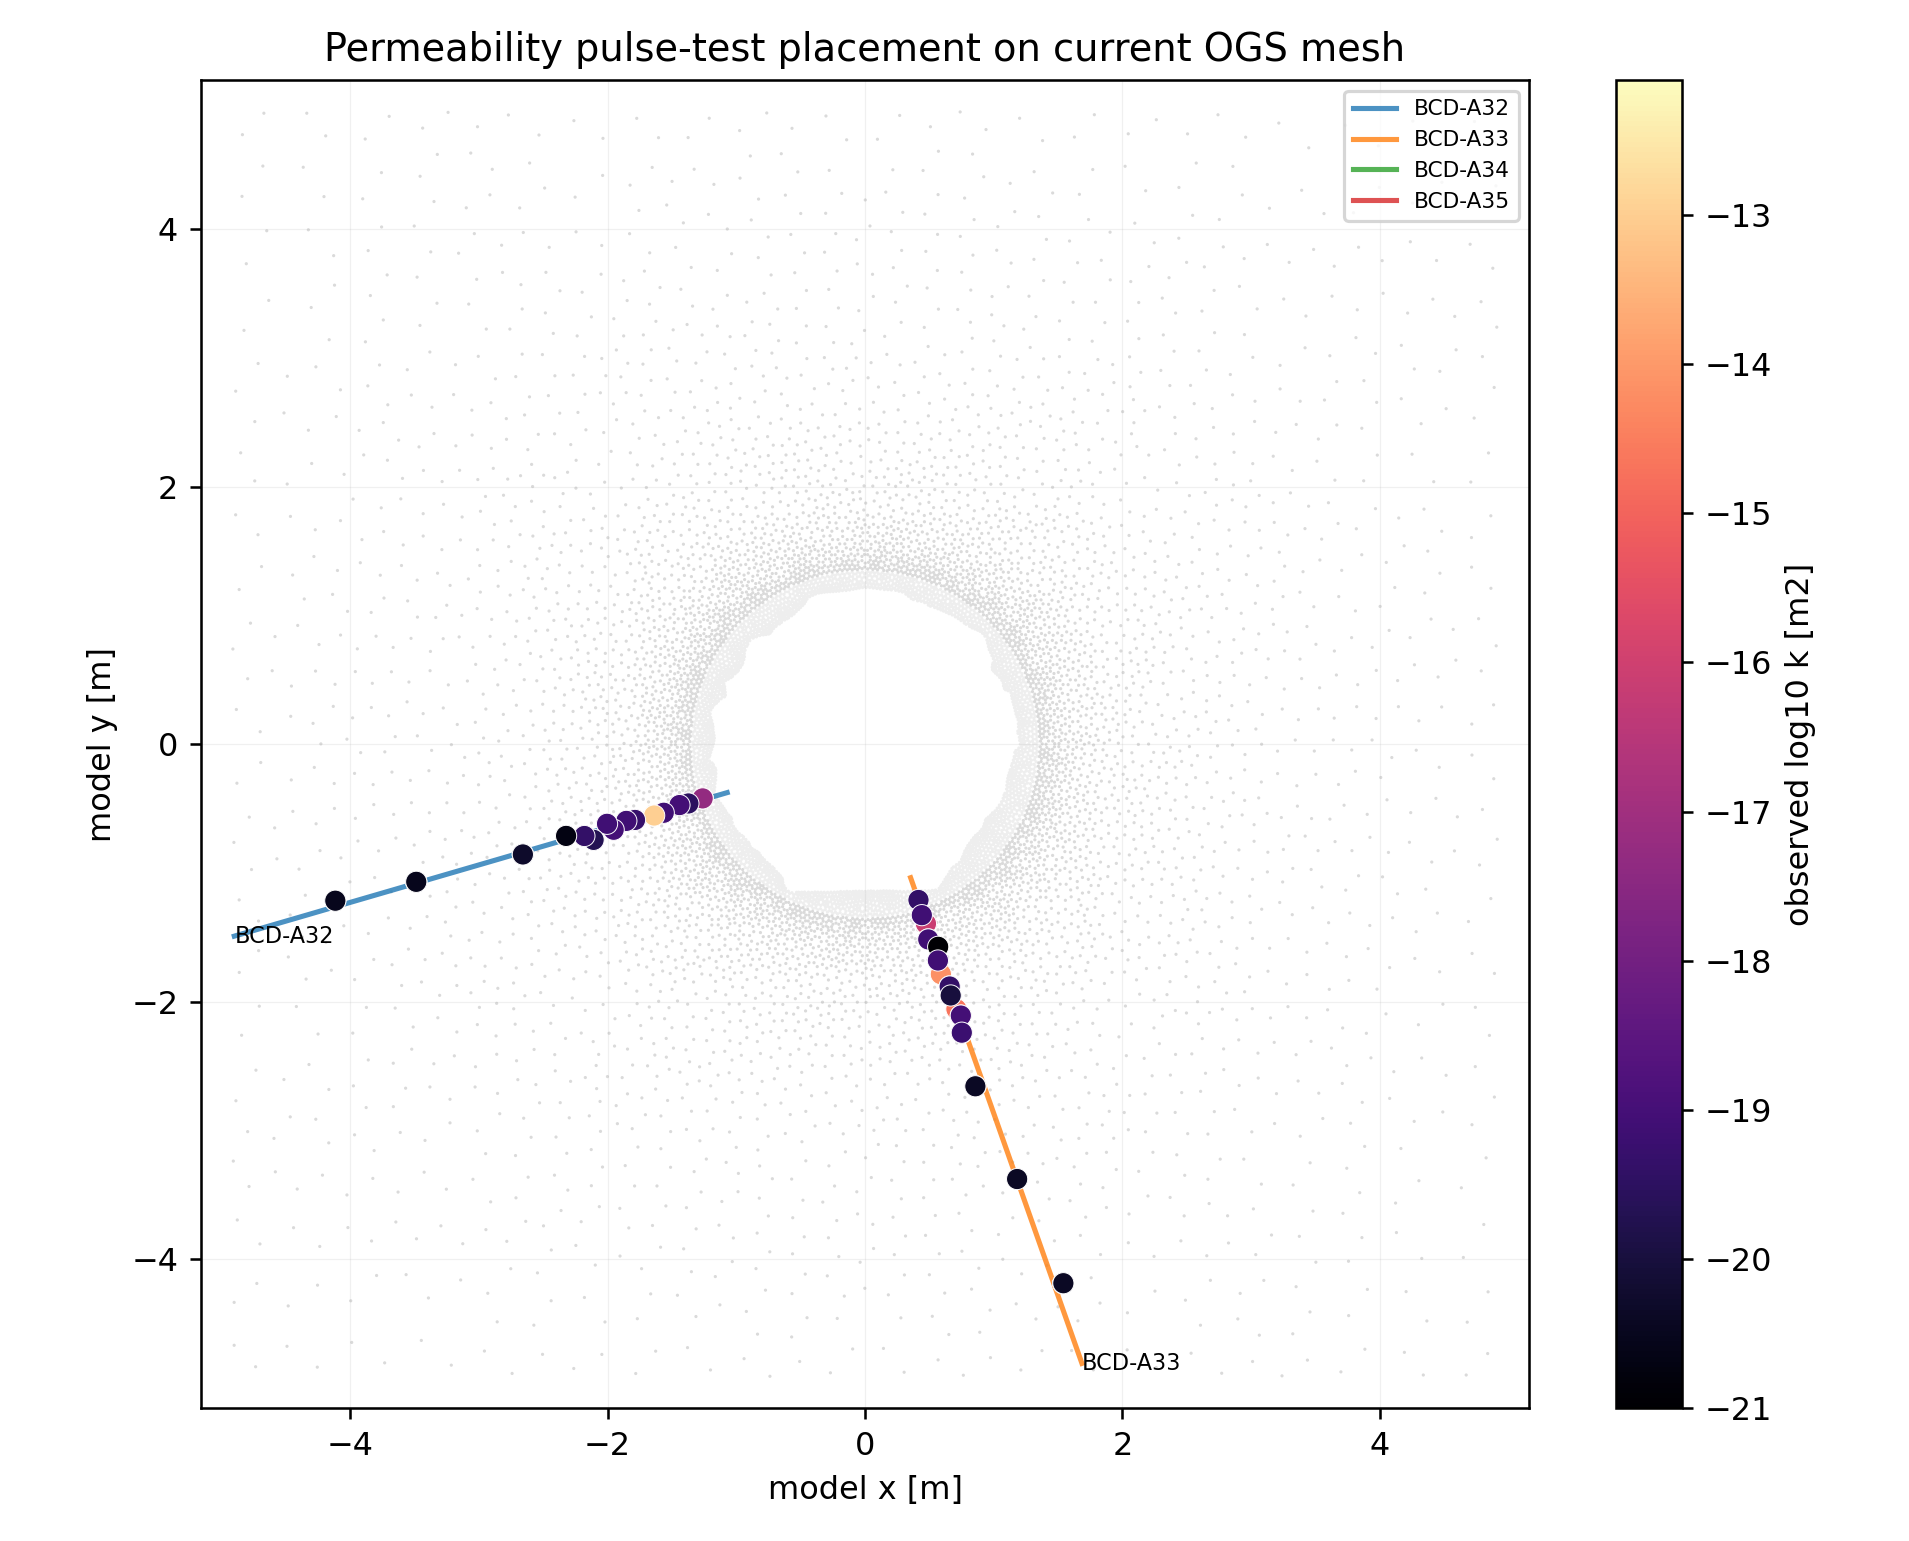
\includegraphics[width=0.86\textwidth]{resources/figures/measurement_permeability_location.png}
  \caption{Location of active direct permeability supports on the current OGS mesh.
  The plotted supports are the BCD-A32 and BCD-A33 pulse-test intervals currently
  usable as direct constraints on \(\KK(\xx)\).}
  \label{fig:permeability-location}
\end{figure}

\paragraph{Time of measurement.}
The processed table contains 204 interpreted rows and 6687 pressure-decay rows.  The
current objective uses the 2024 BCD-A32/A33 rows as quasi-static material evidence.
The 2021 rows are retained as open/closed and historical context, but they are not
part of the current active objective unless their support policy is reopened.

\paragraph{Measured value, units, and model link.}
The interpreted value is permeability in \(\mathrm{m^2}\), used in log10 space.  The
active usable rows span roughly \(-21.0\le\log_{10}(k/\mathrm{m^2})\le -12.10\).
The model link is direct: each row constrains an interval-weighted directional
response of the intrinsic permeability tensor,
\[
  r_i^k
  :=
  \log_{10} k_{i,\mathrm{pred}}
  -
  \log_{10} k_{i,\mathrm{obs}},
  \qquad
  k_{i,\mathrm{pred}}
  =
  \sum_{c\in\mathcal C_i} w_{ic}\,\mathbf e_i^\top\KK_c\mathbf e_i .
\]
Here \(\mathcal C_i\) is the set of OGS cells sampled by row \(i\),
\(w_{ic}\) are support weights, \(\mathbf e_i\) is the interval or borehole-axis unit
direction, and \(\KK_c\) is the cell-wise intrinsic-permeability tensor.
If this comparison is used in a posterior, the likelihood term is built from the
uncertainty-normalized mismatch
\((\log_{10} k_{i,\mathrm{pred}}-\log_{10} k_{i,\mathrm{obs}})/\sigma_i^k\), not
from the plotted permeability value alone.
This residual acts on the material field used by Darcy's law, so permeability
changes also affect pressure diffusion, saturation evolution, NMR water-content
predictions, ERT resistivity predictions, and Taupe/TDR trends.

\paragraph{Uncertainty and reliability.}
The first-pass direct residual uses a 0.5 log10-unit standard deviation and
duplicate-aware weights.  This is a policy choice consistent with the order of the
experimental/evaluation uncertainty, not a proof that every support conflict is
resolved.  Same-support rows can differ by several log10 units, and some tests
appear to jump rapidly between the lowest and highest reported values.  Those
oscillations should be treated first as a quality-control and interpretation gate,
not as independent high-frequency material evolution.  Outlier policy, support
aggregation, endpoint recovery, raw pressure-decay interpretation, and repeat-test
grouping remain active gates.

\subsubsection*{Current computational use.}
With the available source data now, the defensible use is a direct material-field
likelihood on the mapped positive BCD-A32/A33 rows.  The nitrogen pulse-test value
is treated as a noisy scalar observation of the liquid-equivalent intrinsic
permeability used by Darcy flow.  The observation operator is the interval average
of \(\mathbf e^\top\KK\mathbf e\) over the mapped support, evaluated in log10 space.
This is the best current transfer from a gas pulse test to OGS \(\KK\): keep the
reported value as intrinsic permeability in \(\mathrm{m^2}\), keep the gas/slip
interpretation caveat visible, and absorb unresolved gas-to-liquid and support
interpretation errors through a conservative log-space uncertainty and
duplicate-aware weighting
\citep[abstract]{Klinkenberg1941}
\citep[abstract and Secs.~2.2, 3.2]{Marschall2005}
\citep[source files used for the generated support and row summaries]{CDAProvidedMeasurementFiles2025}.

This stream directly constrains only \(\KK(\xx)\) or its varied
parameterization.  It does not independently constrain pressure, saturation,
porosity, retention, or relative permeability.  If the unresolved gas correction,
interval support, tensor direction, or duplicate policy is wrong, an inverse run
will express that error as false spatial heterogeneity in \(\KK\).

\subsubsection*{Grounding questions.}
\revnote{42}{\pdfAnnComment{25}{v ramci vyjasneni toho, co vlastne experimenty
delaji}{The permeability section distinguishes gas pulse-test interpretations from
hydraulic conductivity, relative permeability, saturation, and tensor components.}}
\revnote{43}{\pdfAnnComment{26}{uplne nerozumim, jestli to je pro nas nebo dotaz na
data}{The table keeps both roles: current modelling policy for how to use the
stream, and provider-facing gates for missing gas-correction, support, and metadata
details.}}
\gqGroundingTable{tab:grounding-permeability}
{Grounding questions for direct permeability pulse tests.}
{
\gqPair{gqGate}{Gate}{\qid{Q045} How should tests that rapidly oscillate between the lowest and highest interpreted permeability be understood?}{Treat them as an interpretation and reliability gate before using them as hard
likelihood terms.  The provider should clarify whether the oscillations are raw
pressure-decay fitting instability, leakage or packer effects, gas-slip correction,
support duplication, reprocessing duplicates, or real time evolution.  Until then,
use robust or duplicate-aware weighting, group repeated supports, and avoid reading
the extremes as independent fine-scale \(\KK\) structure.}
}

\begin{figure}[htbp]
  \centering
  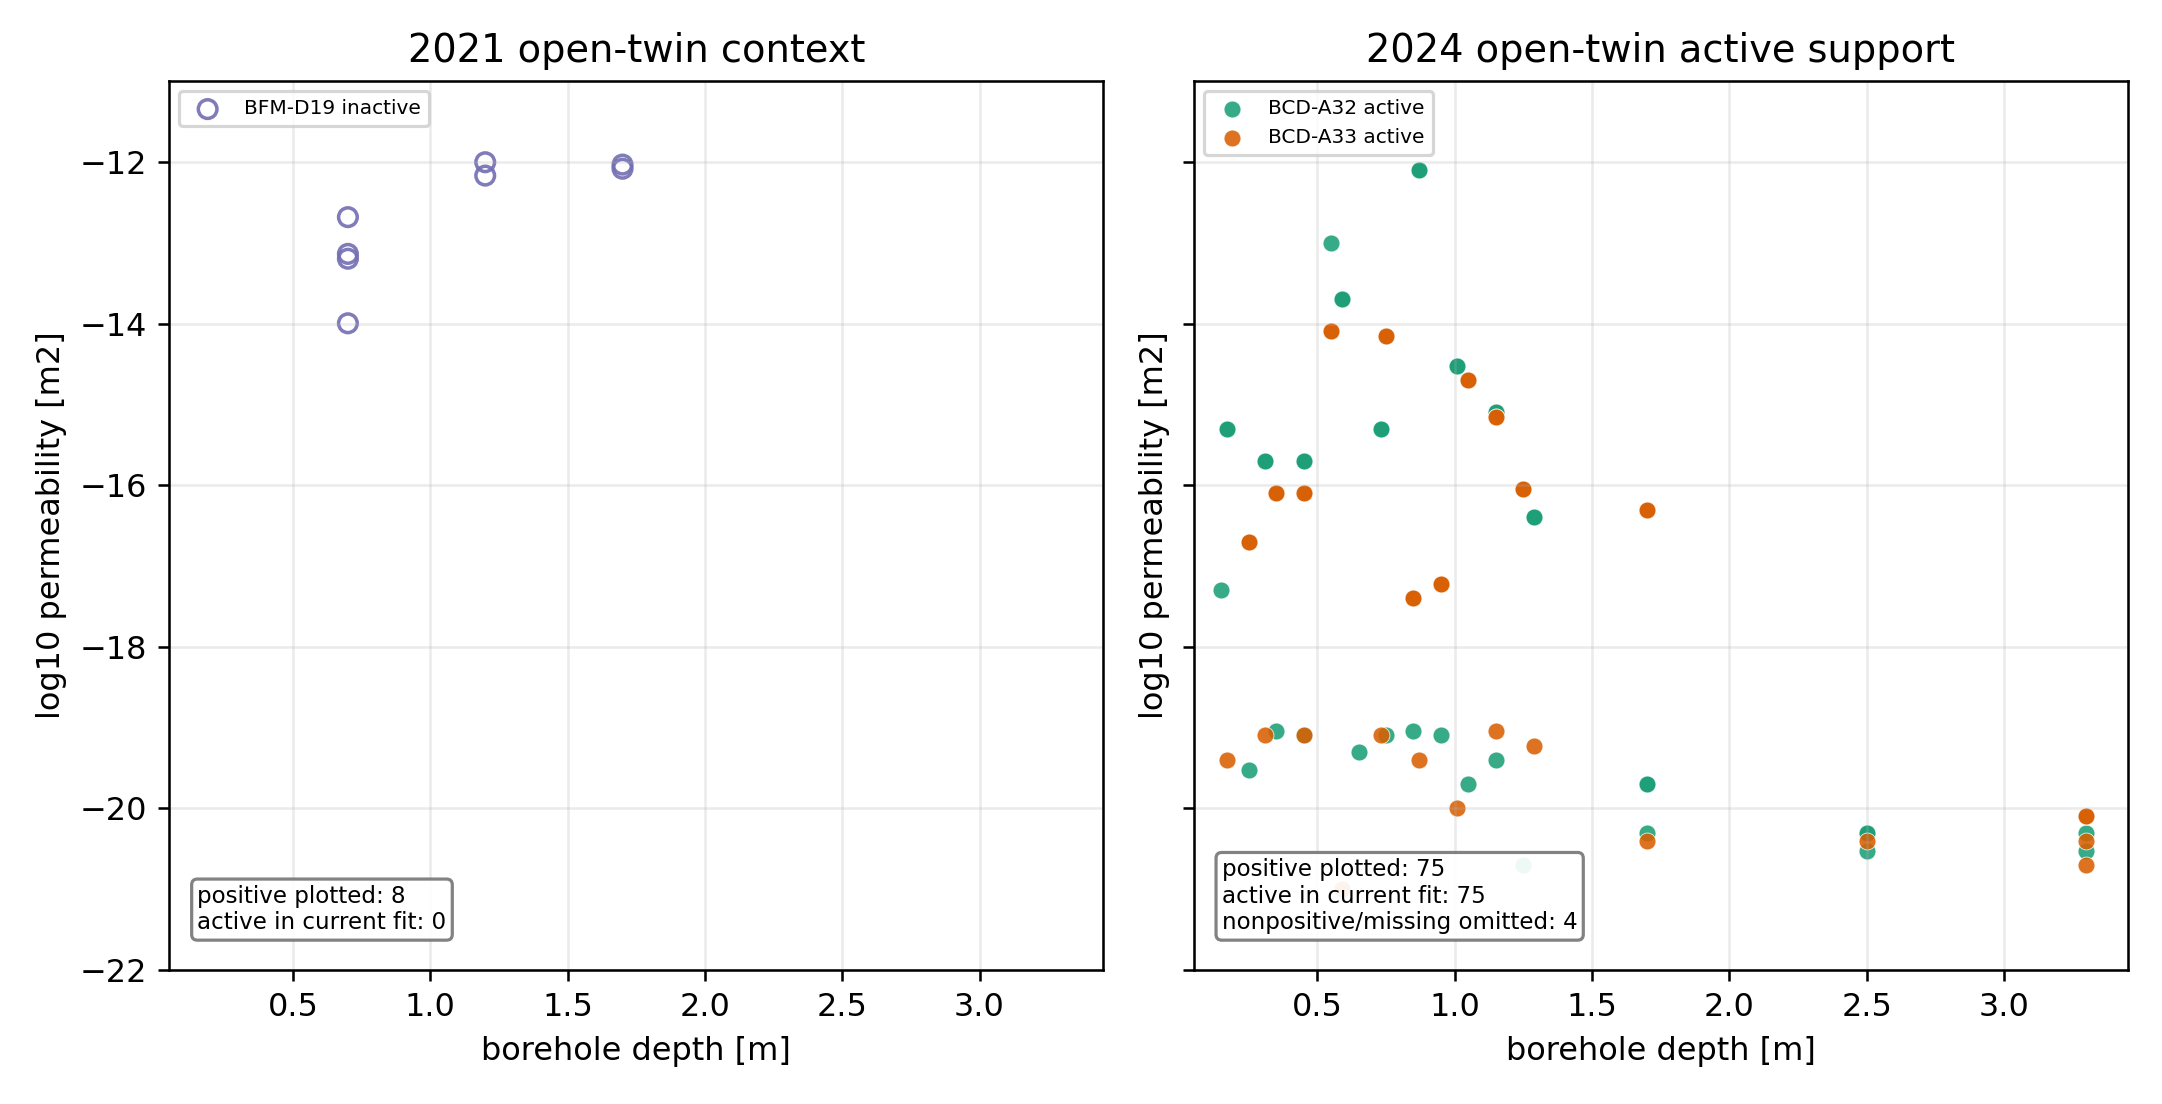
\includegraphics[width=0.98\textwidth]{resources/figures/measurement_permeability_campaigns.png}
  \caption{Open-twin interpreted permeability rows by campaign year.  The 2024
  BCD-A32/A33 values form the active support; earlier rows remain context until
  geometry and support policy are accepted.}
  \label{fig:permeability-campaigns}
\end{figure}

\begin{figure}[htbp]
  \centering
  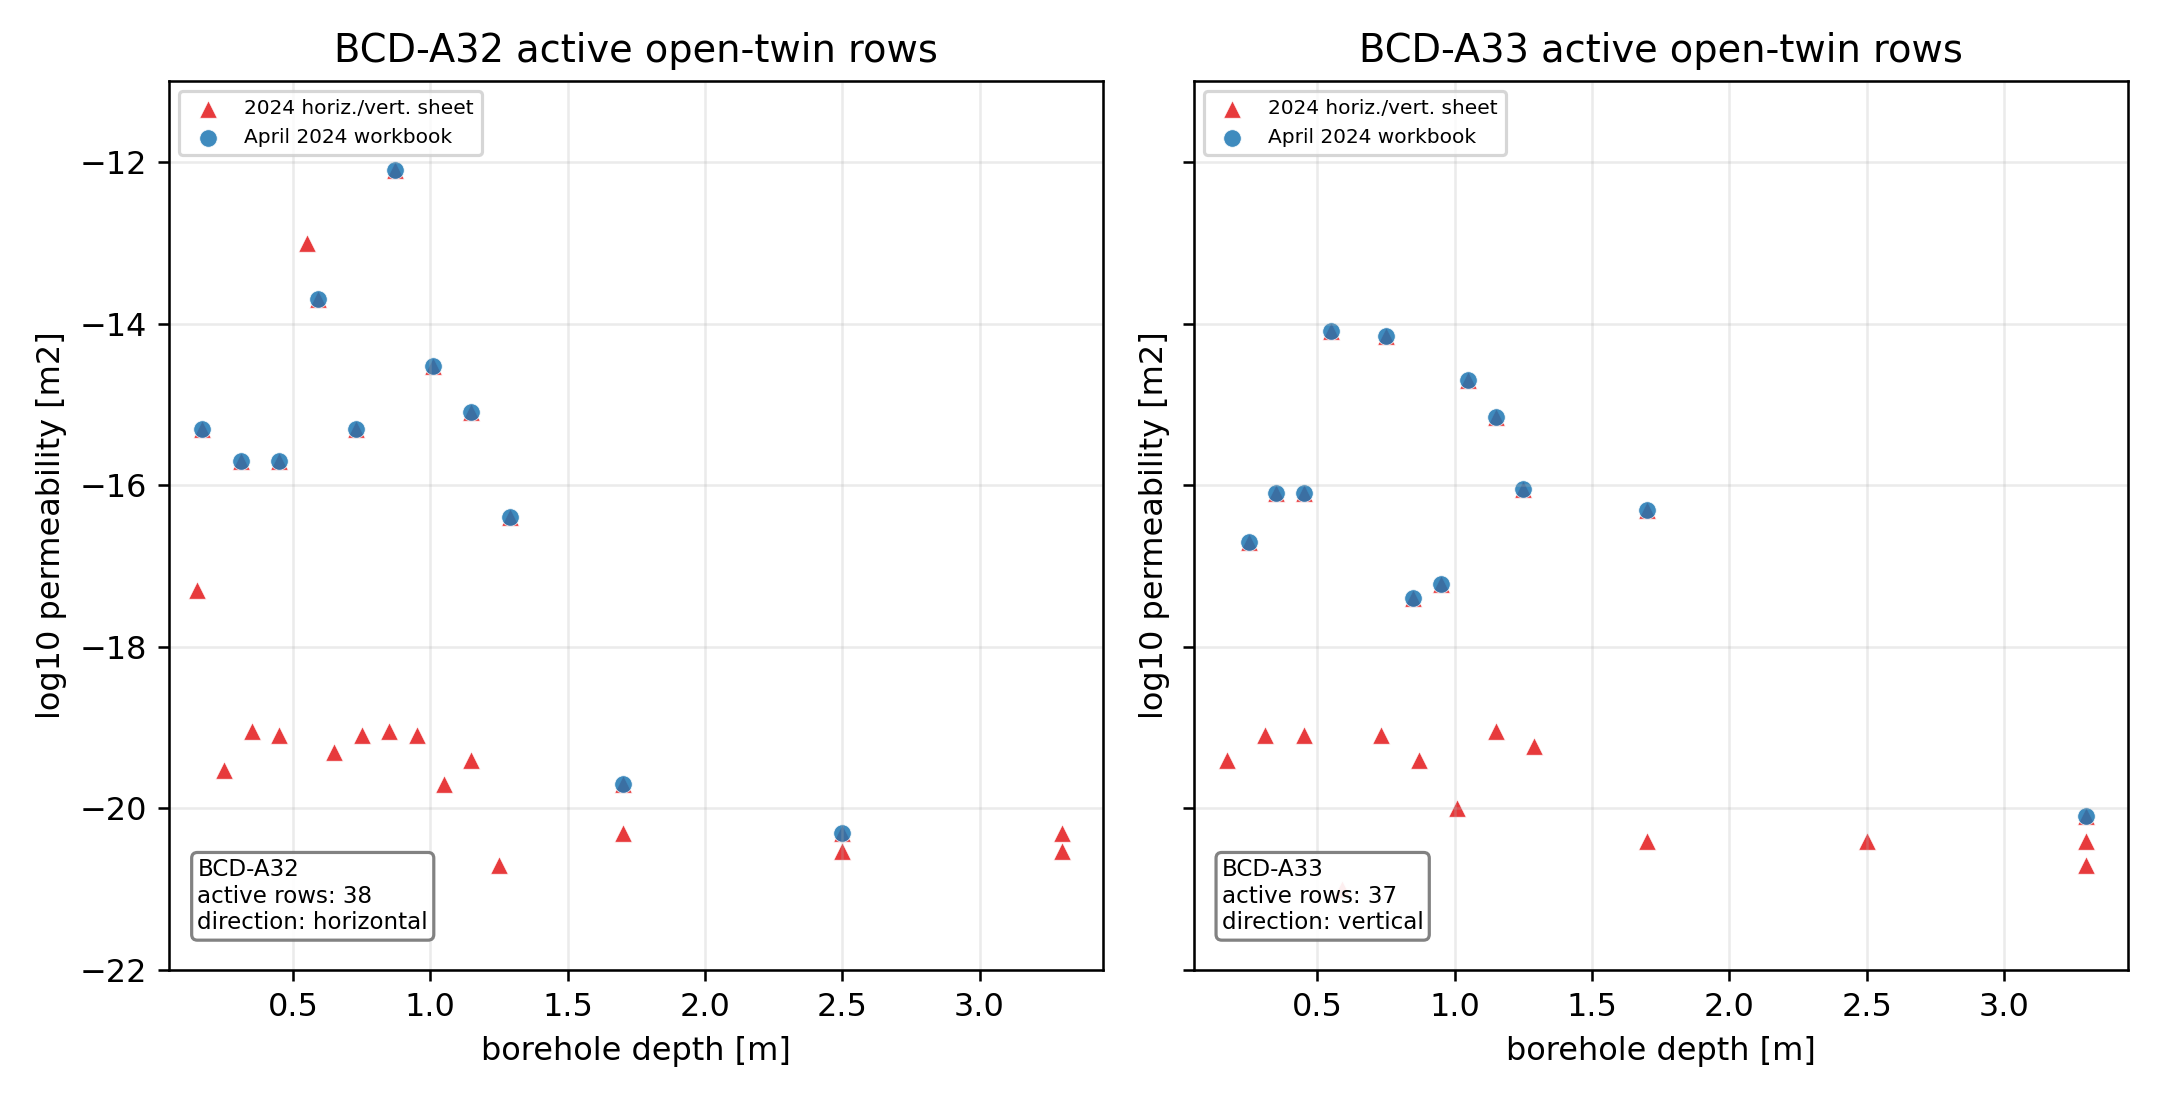
\includegraphics[width=0.98\textwidth]{resources/figures/measurement_permeability_boreholes.png}
  \caption{Active open-twin permeability rows by borehole.  BCD-A32 and BCD-A33
  provide the current horizontal and vertical support families for the direct
  material-field likelihood.}
  \label{fig:permeability-boreholes}
\end{figure}

\FloatBarrier
\section{NMR Water-Content Measurements}
\label{sec:measurement-nmr}

\paragraph{Meaning.}
NMR is the strongest provided water-content evidence, but it is not identical to OGS
liquid saturation.  The weekly and seasonal source tables report volumetric water
content in vol.\% and relaxation-time information.  In claystone the NMR signal can
include mobile pore water and bound or interlayer water.  The model-side quantity
\(\theta=\por\Sl\) is therefore only the mobile-water proxy unless a bound-water
observation model is added
\citep[Sec.~4.2]{WaterContentEDZ2024}
\citep[Secs.~1 and 2.5]{Cui2022DualScaleNMR}
\citep[single-sided NMR technical slides]{NMR2026Email}.

\paragraph{Position in the domain.}
The processed NMR labels are mapped into the two-dimensional OGS frame when
coordinates exist.  Figure~\ref{fig:nmr-location} shows the active and contextual
support positions.  Niche 4 support is relevant for the current model.  Niche 3
campaign rows are retained as experimental context, not as direct observations of
the present slice.

\begin{figure}[htbp]
  \centering
  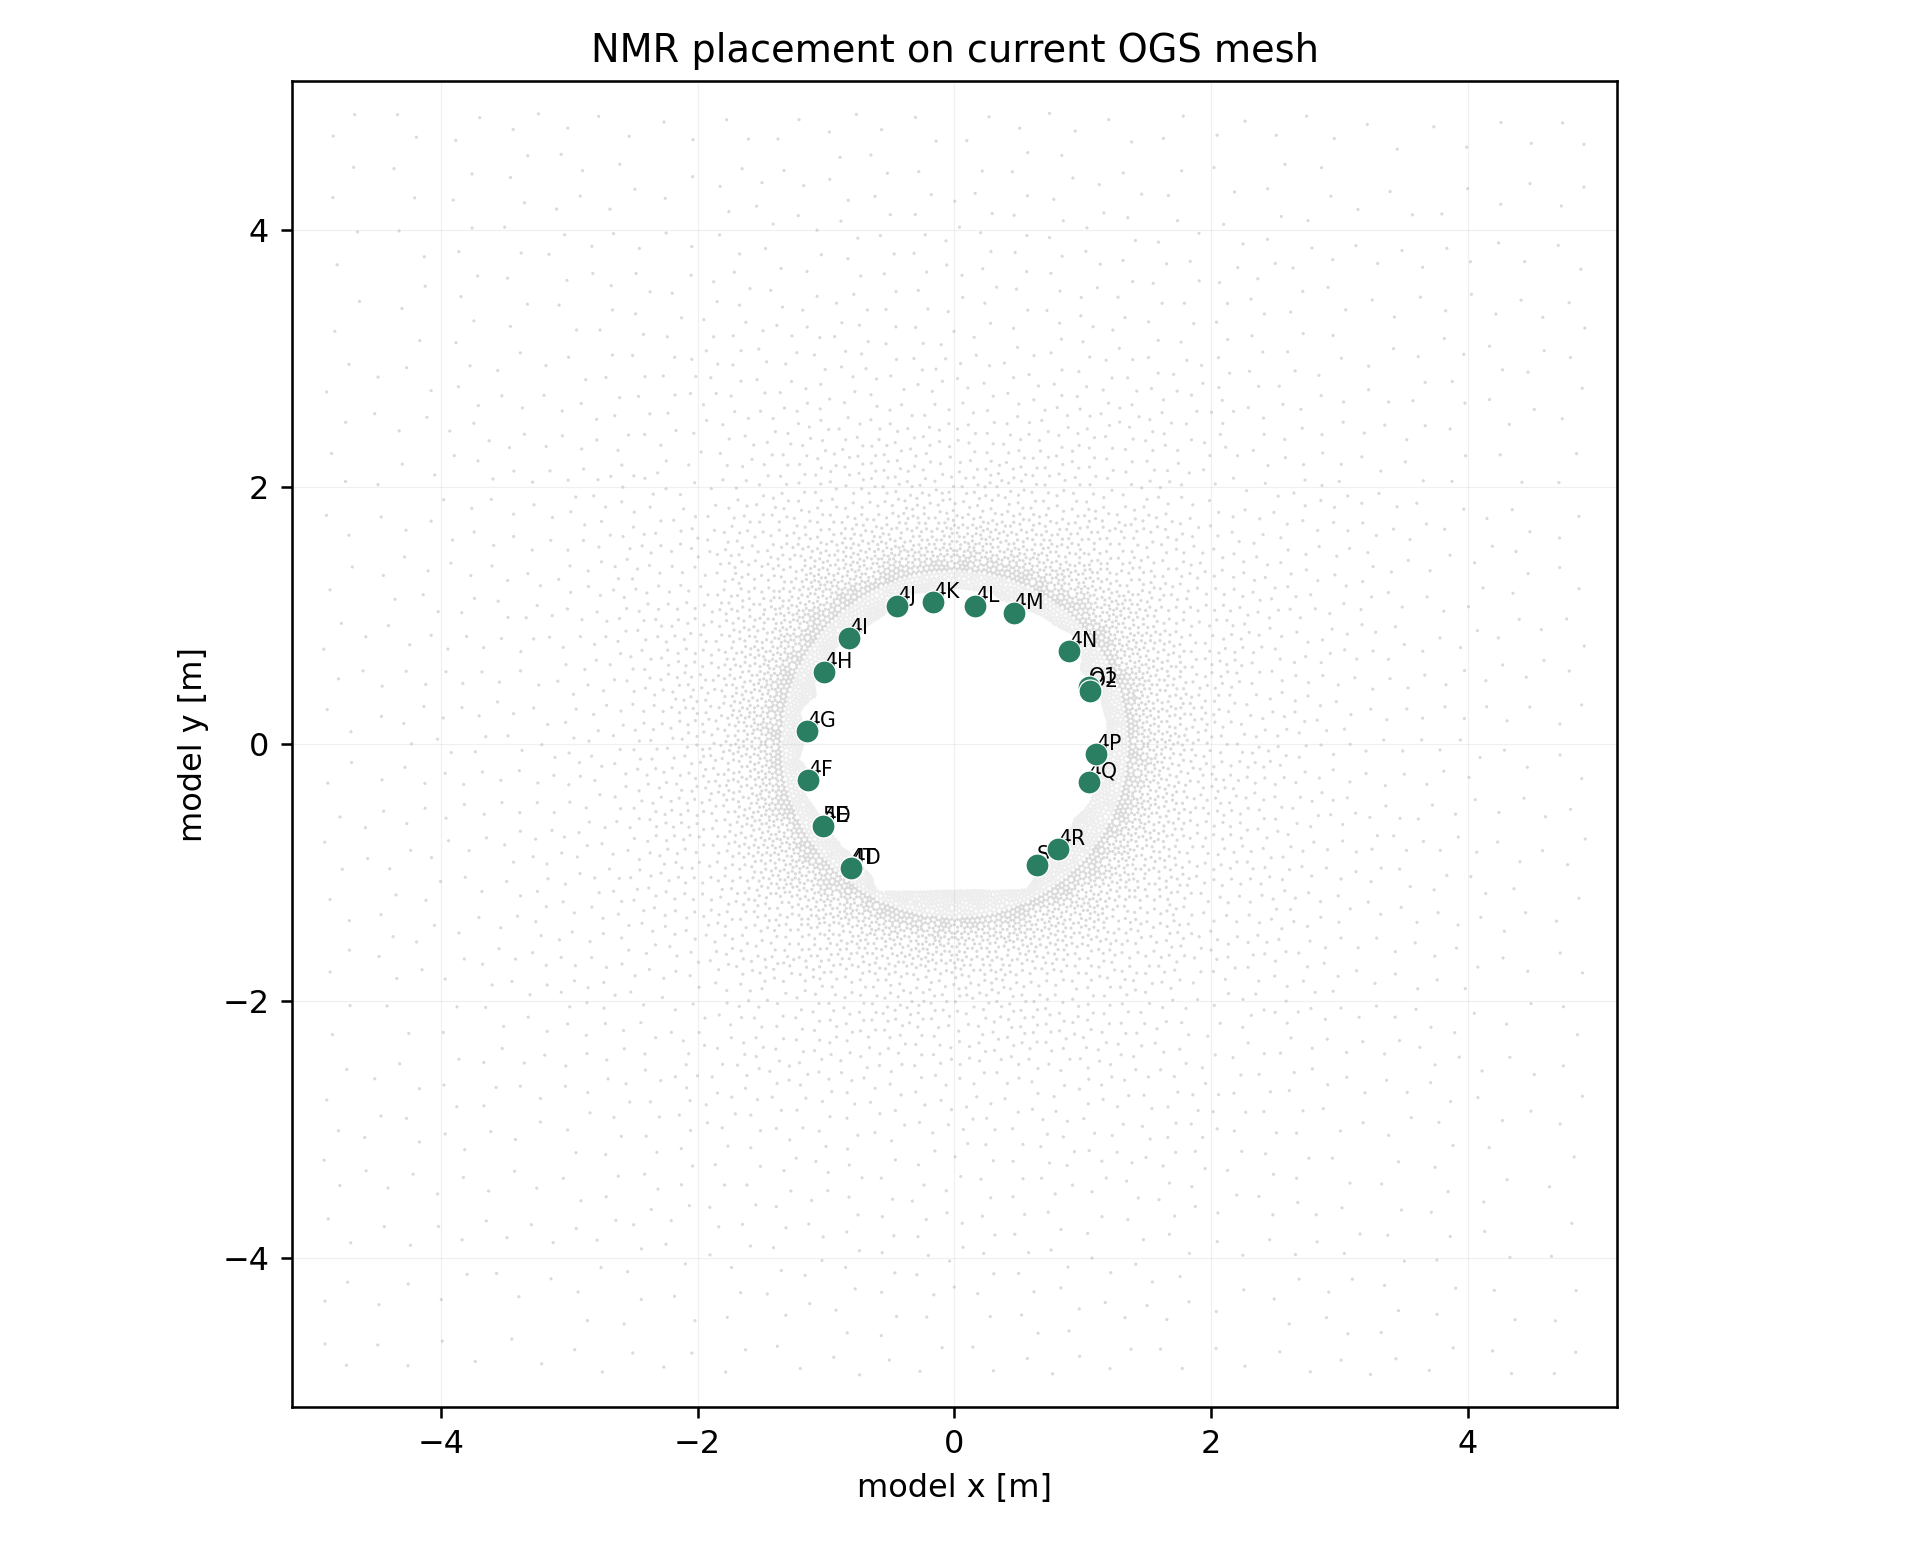
\includegraphics[width=0.86\textwidth]{resources/figures/measurement_nmr_location.png}
  \caption{NMR support positions in the OGS model frame.  These labels define where
  \(\theta=\por\Sl\) is sampled from OGS outputs for raw and trend/anomaly
  comparisons.}
  \label{fig:nmr-location}
\end{figure}

\paragraph{Time of measurement.}
The processed NMR layer contains 170 weekly rows and 294 seasonal profile rows.  The
weekly 4E/4S monitoring covers 2021-10-06 to 2025-09-09, while the seasonal archive
contains campaign profiles for repeated Niche 3 and Niche 4 measurement dates.  The
row-level table keeps caveats such as the 2025 4E detuning period.

\paragraph{Measured value, units, and model link.}
The measured water content is reported in vol.\%; in the model we use the fraction
\(\theta_{\mathrm{obs}}=\mathrm{vol.\%}/100\).  The natural OGS comparison is
\[
  \theta_{\mathrm{NMR}}^{\mathrm{obs}}
  =
  \theta_{\mathrm{mobile}}
  +\theta_{\mathrm{bound}}
  +\epsilon_{\mathrm{NMR}},
  \qquad
  \theta_{\mathrm{mobile}}^{\mathrm{model}}
  \approx
  \por\Sl .
\]
Here \(\theta_{\mathrm{bound}}\) represents NMR-visible bound or interlayer water not
carried as an OGS mobile-liquid state, and \(\epsilon_{\mathrm{NMR}}\) represents
measurement and observation-model error.
The active objective uses raw absolute \(\theta\) on the accepted mapped subset.
The preferred next policy is a within-label anomaly residual, because it removes
constant station or bound-water offsets before comparing model and measurement
changes.

\paragraph{Uncertainty and reliability.}
The bound-water check shows why absolute NMR must remain provisional: with fixed
\(\por=0.105\), 315 of 464 NMR target rows exceed the maximum possible value of
\(\por\Sl\) if interpreted as mobile water.  In the usable current-mesh subset, 162
of 287 rows exceed the same bound.  Reported confidence intervals and an uncertainty
floor are useful, but they do not solve the semantic difference between total
NMR-visible water and mobile OGS liquid.

\subsubsection*{Current computational use.}
With the available source data now, NMR can be used as a provisional
water-content-state comparison, preferably as a within-label trend/anomaly
likelihood rather than a raw absolute likelihood.  The current OGS state supplies
\(\theta_{\mathrm{model}}=\por\Sl\).  The NMR value should be treated as total
NMR-visible water unless the source processing proves a mobile/free-water cut.
The safest current observation model is therefore
\[
  \theta_{\mathrm{NMR}}^{\mathrm{obs}}
  =
  \por\Sl
  + b_{\mathrm{label}}
  + b_{\mathrm{campaign}}
  + \epsilon ,
\]
or the equivalent anomaly model after subtracting stable label/campaign offsets.
This matches the provided NMR evidence that many rows exceed the fixed OGS porosity
and the cited clay/NMR caveat that NMR-visible water can include bound or
interlayer water
\citep[Sec.~4.2]{WaterContentEDZ2024}
\citep[Secs.~1 and 2.5]{Cui2022DualScaleNMR}
\citep[NMR source files used for the generated row summaries]{CDAProvidedMeasurementFiles2025}.

The inverse role is to constrain pressure/saturation evolution after the boundary
and permeability field drive \(\Sl\).  NMR alone cannot separate porosity,
retention, mobile fraction, and bound-water offset.  Releasing those at the same
time without priors would let the inverse problem fit the same water-content
residual in several physically different ways.

\subsubsection*{Grounding questions.}
\revnote{44}{\pdfAnnComment{27}{!!!}{The NMR value meaning remains a gate: the paper
treats the supplied value as total NMR-visible volumetric water content until the
provider confirms a mobile/free-water cut.}}
\revnote{45}{\pdfAnnComment{28}{!!!}{The NMR-to-OGS link is deliberately not raw
saturation.  The current operator uses \(\theta=\por\Sl\) only with bias or anomaly
terms.}}
\revnote{46}{\pdfAnnComment{29}{asi spise pro nas?}{The bound-water offset is a
modelling gate: it can be treated as a nuisance offset only if collaborators confirm
that it is stable by label, campaign, depth, or material class.}}
\revnote{47}{\pdfAnnComment{30}{asi spise pro nas?}{The paper blocks post-processing
bound water from OGS saturation unless a supported relation is supplied.}}
\revnote{48}{\pdfAnnComment{31}{asi spise pro nas}{The NMR full-grounding row lists
the missing units, mobile-water cut, calibration, detuning flags, offsets,
coordinates, uncertainty conversion, and \( \theta_{\mathrm{obs}}>\por \) policy.}}
\gqGroundingTable{tab:grounding-nmr}
{Grounding questions for NMR water-content measurements.}
{
\gqPair{gqGate}{Gate}{\qid{Q050} What exactly does the supplied NMR value measure?}{Treat it as total NMR-visible volumetric water content for now; provider
confirmation is needed for any mobile/free-water interpretation.}
\gqPair{gqPolicy}{Policy}{\qid{Q051} How should NMR be linked to OGS output now?}{Compare to \(\theta=\por\Sl\) only through a bias or anomaly observation model,
not as raw mobile water everywhere.}
\gqPair{gqGate}{Gate}{\qid{Q052} Can bound/interlayer water be anchored simply?}{Yes, if collaborators confirm that the bound-water offset is approximately
constant by label, material class, depth, or campaign; then it can be a nuisance
offset rather than an OGS state.}
\gqPair{gqGate}{Gate}{\qid{Q053} Could bound water be post-processed from OGS saturation?}{Only if a supported relation is supplied; otherwise it should remain a constant or
hierarchical observation offset, not a fitted material field.}
\gqPair{gqGate}{Gate}{\qid{Q054} What would fully ground NMR residuals?}{Source units, T2/mobile-water cut policy, calibration and detuning flags,
label/campaign offsets, support coordinates, confidence-interval conversion, and a
rule for rows where \(\theta_{\mathrm{obs}}>\por\).}
}

\begin{figure}[htbp]
  \centering
  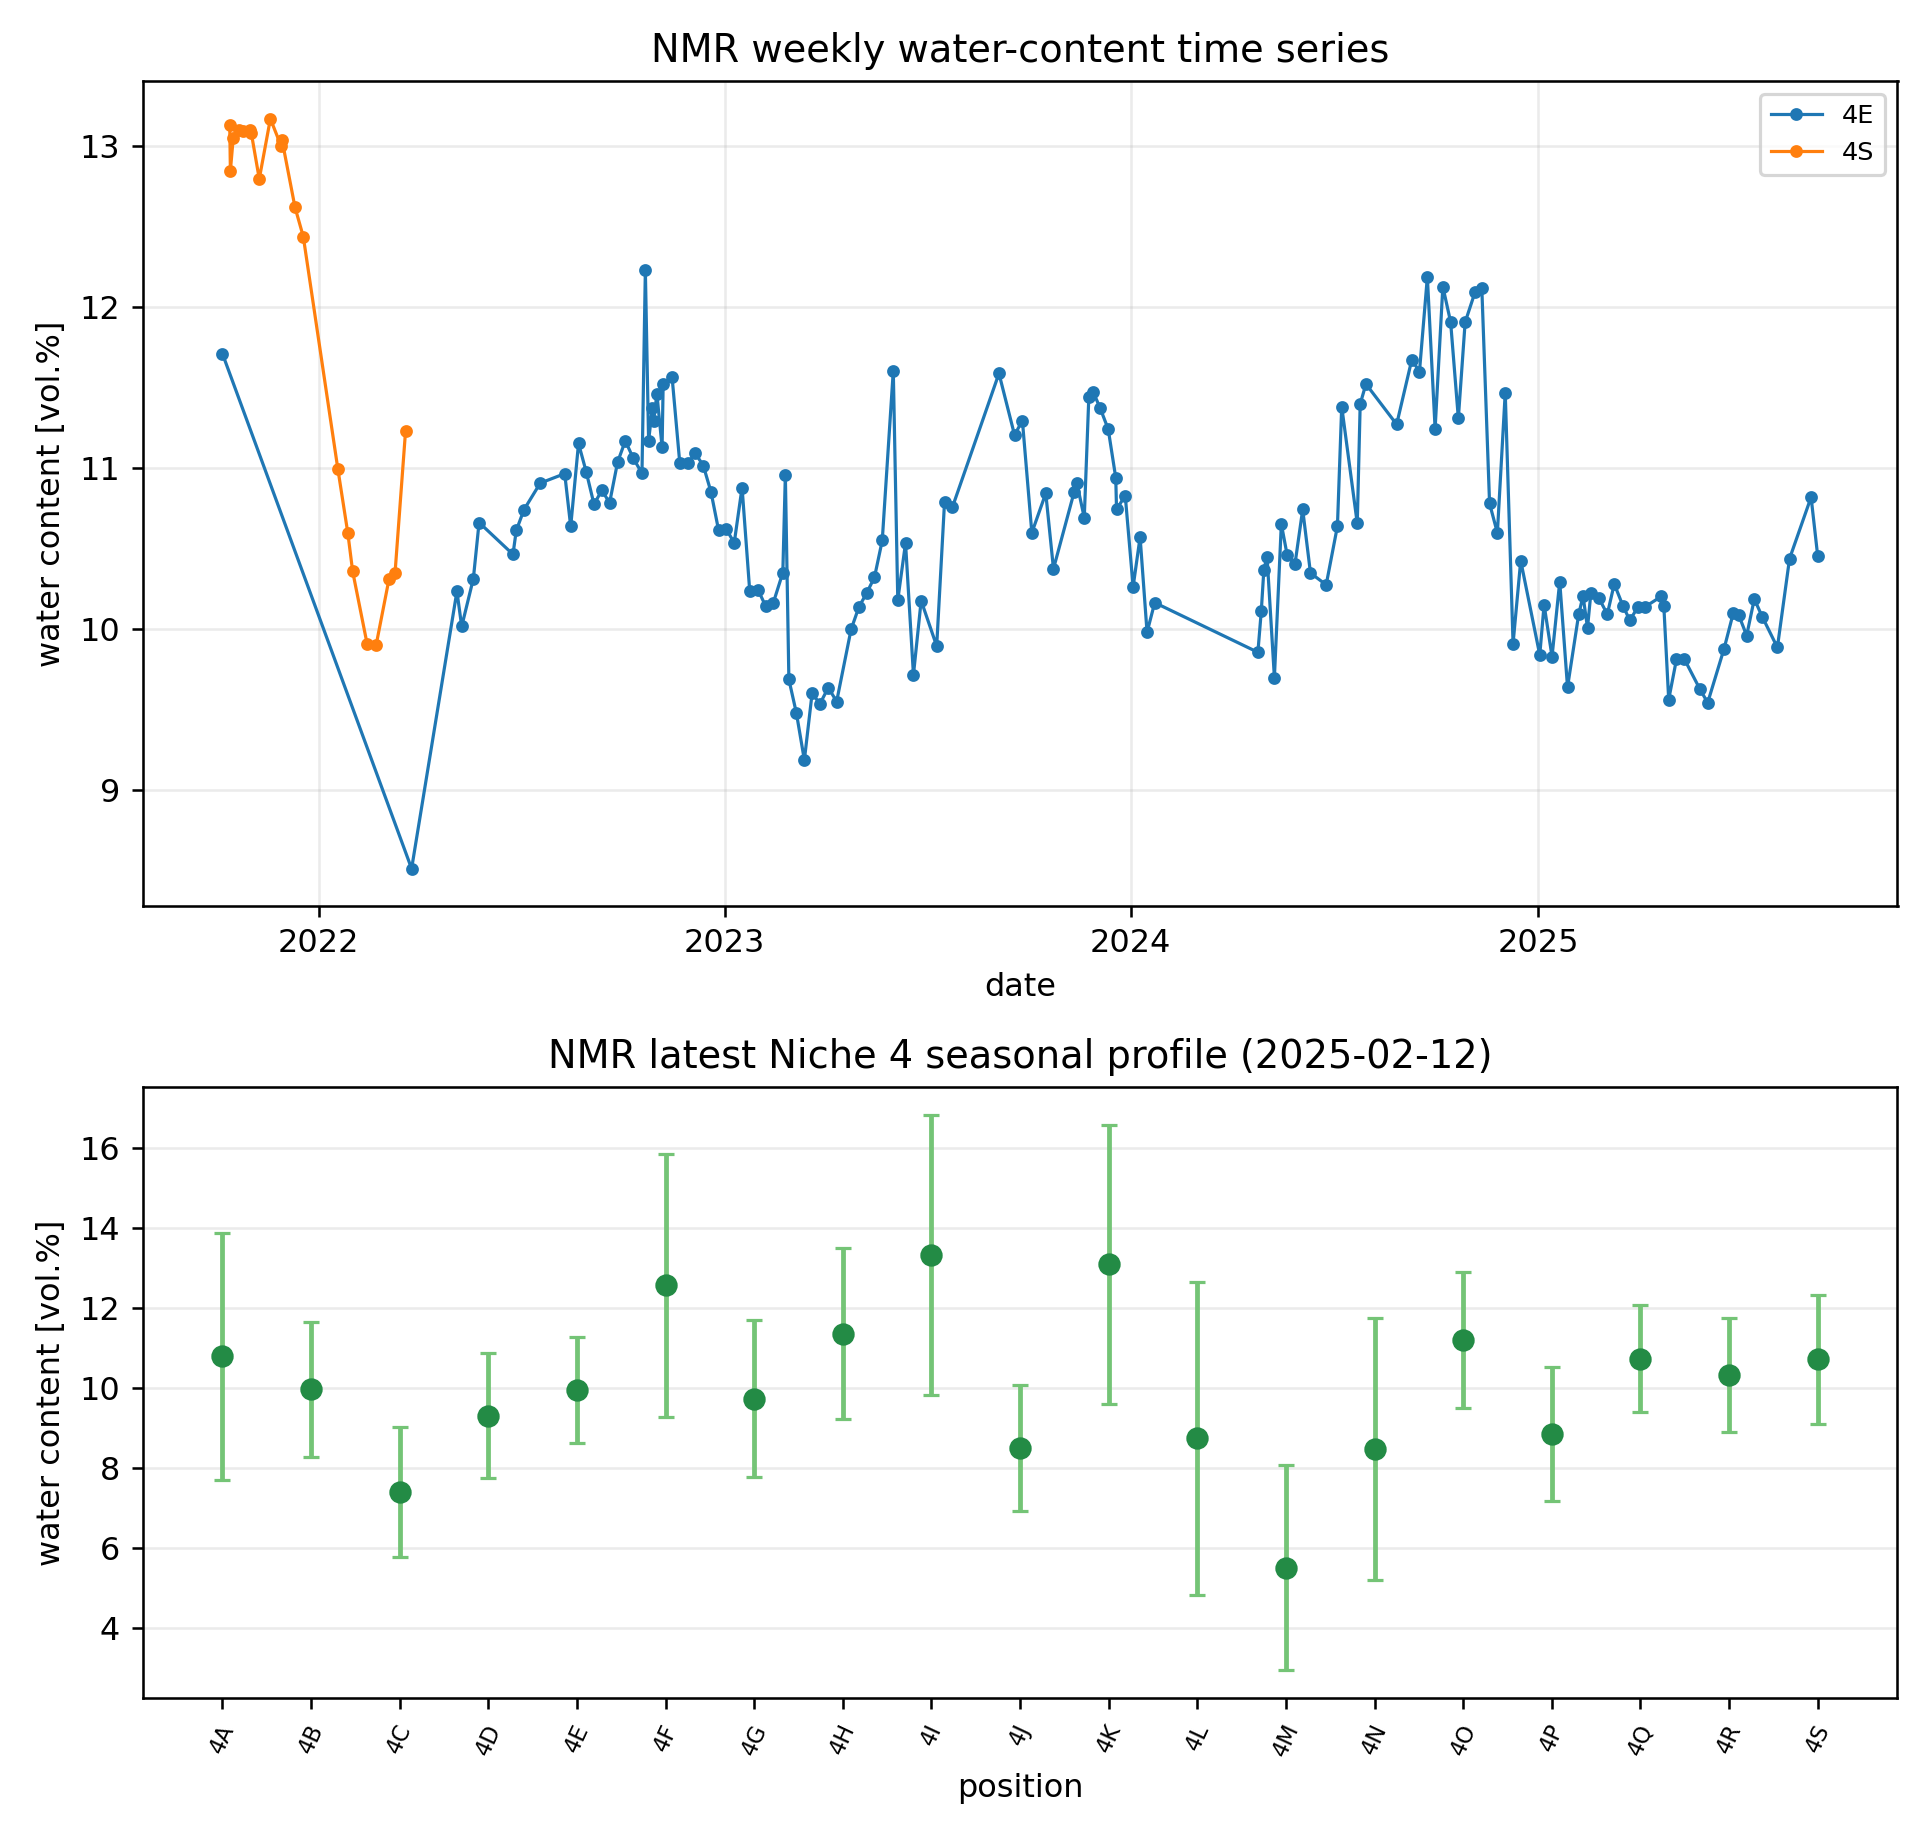
\includegraphics[width=0.98\textwidth]{resources/figures/measurement_nmr_data.png}
  \caption{NMR measured-data visualisation.  The upper panel shows weekly 4E/4S
  water-content histories.  The lower panel shows a seasonal Niche 4 profile with
  confidence intervals.  Values are total NMR-visible water content in vol.\%.}
  \label{fig:nmr-data}
\end{figure}

\FloatBarrier
\section{ERT Resistivity Measurements}
\label{sec:measurement-ert}

\paragraph{Meaning.}
ERT measures an electrical response that is inverted to a resistivity field.  It is
not a direct measurement of saturation, pressure, or permeability.  The physically
defensible model link is a forward observation operator: OGS predicts pressure and
saturation; saturation is converted to a water-content proxy; water content is
converted through the current empirical resistivity relation; the result is projected to
the ERT support.  Classical Archie-type relations motivate the structure, but
claystone requires CD-A-specific calibration because surface conductivity, bound water,
fractures, and anisotropy can contribute to electrical conduction
\citep[pp.~54--56]{Archie1942}
\citep[abstract and Secs.~2--4]{Revil1998ShalySands}
\citep[Secs.~4.1--4.3]{WaterContentEDZ2024}.

\paragraph{Position in the domain.}
The current comparison uses the open-niche ERT archive and the open electrode
example file.  That archive contains a reference inverted mesh with 5966 triangular
cells and 3126 points.  The provisional projection transforms raw ERT coordinates by
\(x_{\mathrm{model}}=x_{\mathrm{ERT}}\) and
\(y_{\mathrm{model}}=z_{\mathrm{ERT}}+500\,\mathrm{m}\).  It maps 4676 cells inside an
OGS cell, with 2035 cells both inside an OGS cell and inside the approximate
near-niche support.  The closed-electrode example is retained as source context,
but it is not used for the current open-niche OGS comparison.

\begin{figure}[htbp]
  \centering
  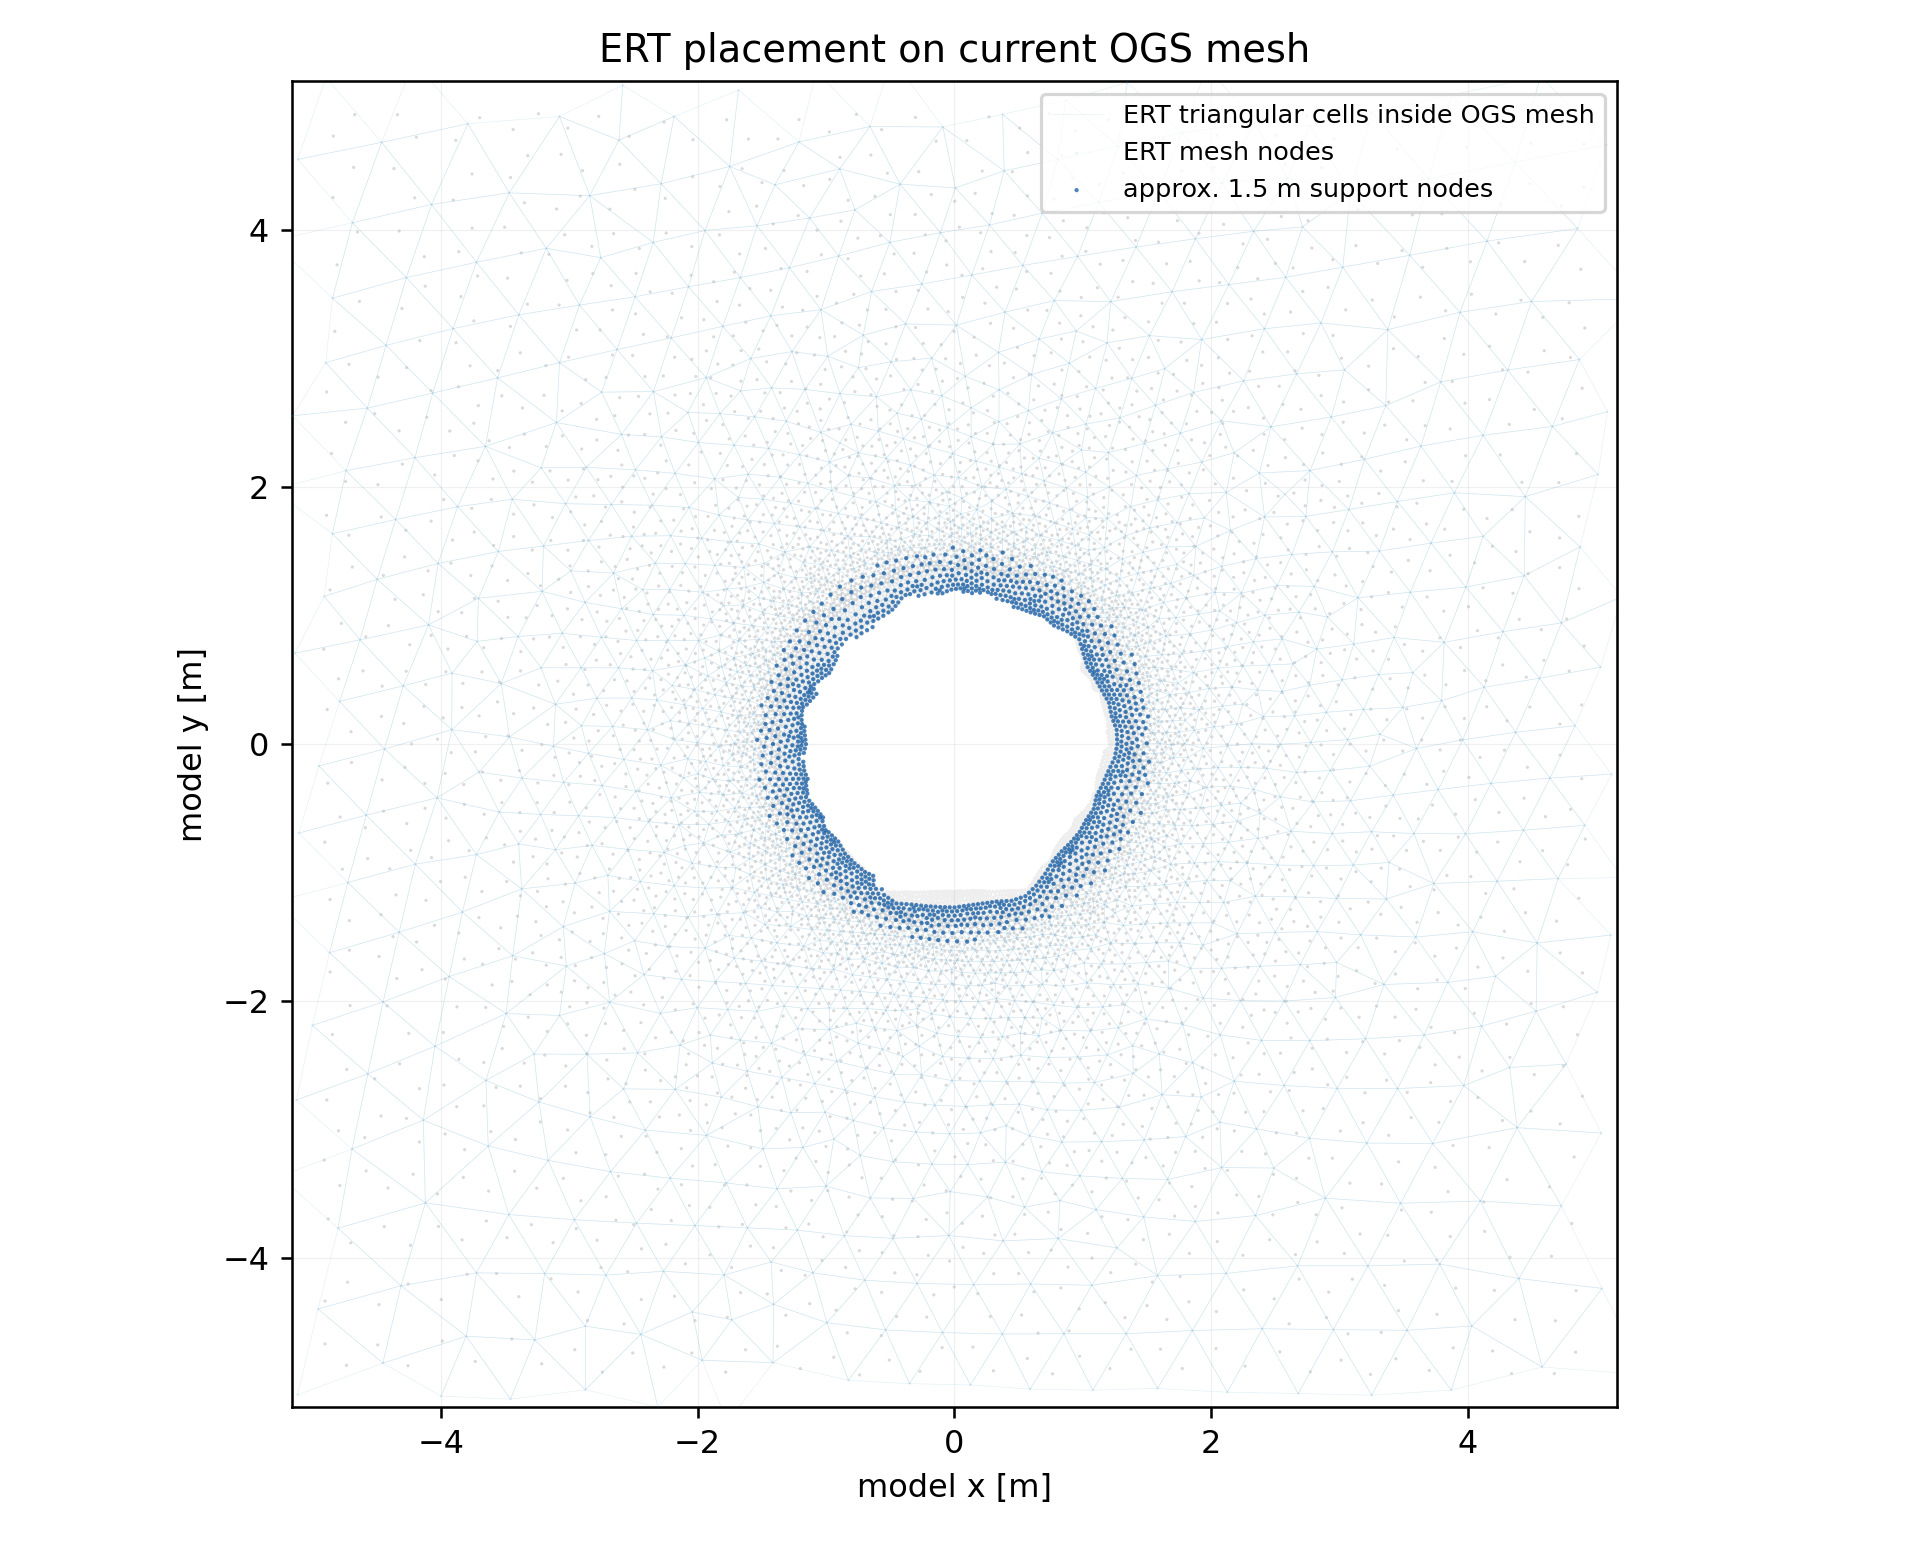
\includegraphics[width=0.86\textwidth]{resources/figures/measurement_ert_location.png}
  \caption{Projected ERT mesh support in the OGS frame.  The darker subset indicates
  the current approximate near-niche support used for diagnostics before the exact
  support mask is accepted.}
  \label{fig:ert-location}
\end{figure}

\paragraph{Time of measurement.}
The processed ERT inventory contains 1691 timestep entries from 2019-11-01 to
2024-12-31.  Of these entries, 1675 have matching VTK fields and 16 are missing a
matching VTK member.  The archive therefore has dense temporal information, but it
must be matched to OGS output times through an explicit tolerance.

\paragraph{Measured value, units, and model link.}
The comparison should be made in log-resistivity, for example
\[
  \Sl(\xx,t)
  \longrightarrow
  \theta(\xx,t)=\por\Sl(\xx,t)
  \longrightarrow
  \rho_{\Omega\mathrm{m}}(\xx,t)
  =
  1.108\,\theta(\xx,t)^{-1.58}
  \longrightarrow
  \mathcal O_{\mathrm{ERT}}[\rho_{\Omega\mathrm{m}}],
\]
followed by
\[
  r^{\mathrm{ERT}}
  :=
  \log_{10}\rho_{\mathrm{pred}}
  -
  \log_{10}\rho_{\mathrm{ERT}} .
\]
Here \(\rho_{\Omega\mathrm{m}}\) denotes electrical resistivity in
\(\Omega\,\mathrm{m}\), and \(\mathcal O_{\mathrm{ERT}}\) denotes the projection or
aggregation from the OGS field to the inverted ERT support.
The empirical relation is the current provisional default over the calibrated range
\(0.01\le\theta\le0.18\).  It should not be interpreted as a universal
Opalinus-Clay water-content law.

\paragraph{Uncertainty and reliability.}
ERT remains diagnostic.  The unresolved gates are the exact coordinate transform,
the exact tunnel/niche support mask, the 35 cm rock-depth convention, and the
uncertainty/correlation model.  Without a covariance or aggregation rule, dense
neighbouring inversion cells would overweight one physical field image.
The processed VTK products are enough for diagnostics, but raw ERT measurements are
needed for faster controlled tests, covariance checks, bad-electrode screening, and
reprocessing.  If the full archive is too large to transfer first, the practical
minimum request is the raw electrode-data package for the first two years starting
from the 2019-11-01 survey.

\subsubsection*{Current computational use.}
With the available source data now, ERT should remain a diagnostic field and
candidate future likelihood.  The best current operator is the explicit
post-processing chain
\[
  \Sl \rightarrow \theta=\por\Sl
  \rightarrow \rho_{\Omega\mathrm{m}}=1.108\,\theta^{-1.58}
  \rightarrow \mathcal O_{\mathrm{ERT}}\rho
  \rightarrow \log_{10}\rho ,
\]
using the provisional coordinate transform and near-niche mask only for
diagnostics.  This keeps the empirical CD-A water--resistivity relation separate
from the OGS hydraulic state, and it prevents the inverted ERT mesh from being
mistaken for independent point measurements
\citep[pp.~54--56]{Archie1942}
\citep[abstract and Secs.~2--4]{Revil1998ShalySands}
\citep[Secs.~4.1--4.3]{WaterContentEDZ2024}
\citep[ERT source files used for the generated field summaries]{CDAProvidedMeasurementFiles2025}.

For inversion, ERT mainly constrains the saturation/water-content pattern and
therefore tests permeability, boundary forcing, and retention indirectly.  Its
dense cells share electrodes, inversion regularization, and projection errors.
Without aggregation or covariance, ERT would dominate the objective numerically
while adding much less independent information than the row count suggests.

\subsubsection*{Grounding questions.}
\revnote{49}{\pdfAnnComment{32}{!!!}{The ERT section keeps bound/interlayer water
and clay surface conduction as explicit gates before absolute water-content
inversion.}}
\revnote{50}{\pdfAnnComment{33}{!!!}{The ERT section keeps electrical anisotropy as
a gate because bedding, fractures, and permeability anisotropy may affect the
electrical response, but no accepted operator is available yet.}}
\gqGroundingTable{tab:grounding-ert}
{Grounding questions for ERT resistivity measurements.}
{
\gqPair{gqGate}{Gate}{\qid{Q056} Is the Archie-type water-content--log-resistivity fit global, or only a local empirical relation?}{Treat
\(\rho_{\Omega\mathrm{m}}=1.108\,\theta^{-1.58}\) as the current local
CD-A empirical fit between water content and log-resistivity, not as a global
Archie law.  Expert confirmation is needed on its calibrated range, whether
\(\theta=\por\Sl\) is the right water-content proxy, and whether separate
calibrations are needed for bound water, clay surface conduction, pore-fluid
chemistry, fractures, or anisotropy.}
\gqPair{gqGate}{Gate}{\qid{Q057} Does bound water conduct like free water?}{Not settled; clay surface conduction and bound/interlayer water are explicit gates
before absolute water-content inversion.}
\gqPair{gqGate}{Gate}{\qid{Q058} Does electrical anisotropy matter?}{Possibly; bedding, fractures, and permeability anisotropy may affect electrical
response, but no accepted electrical-anisotropy operator exists for this workflow.}
\gqPair{gqGate}{Gate}{\qid{Q086} Can we obtain raw ERT data for all campaigns, or at least the first two years?}{Request raw electrode measurements, timestamps, array configurations, reciprocal or
error estimates, current/voltage data, inversion settings, and bad-electrode flags
for all ERT campaigns.  If that is too large for the first transfer, request the
same package for the initial two-year window beginning with the 2019-11-01 survey,
so time-shift and likelihood tests can be run quickly.}
}

\begin{figure}[htbp]
  \centering
  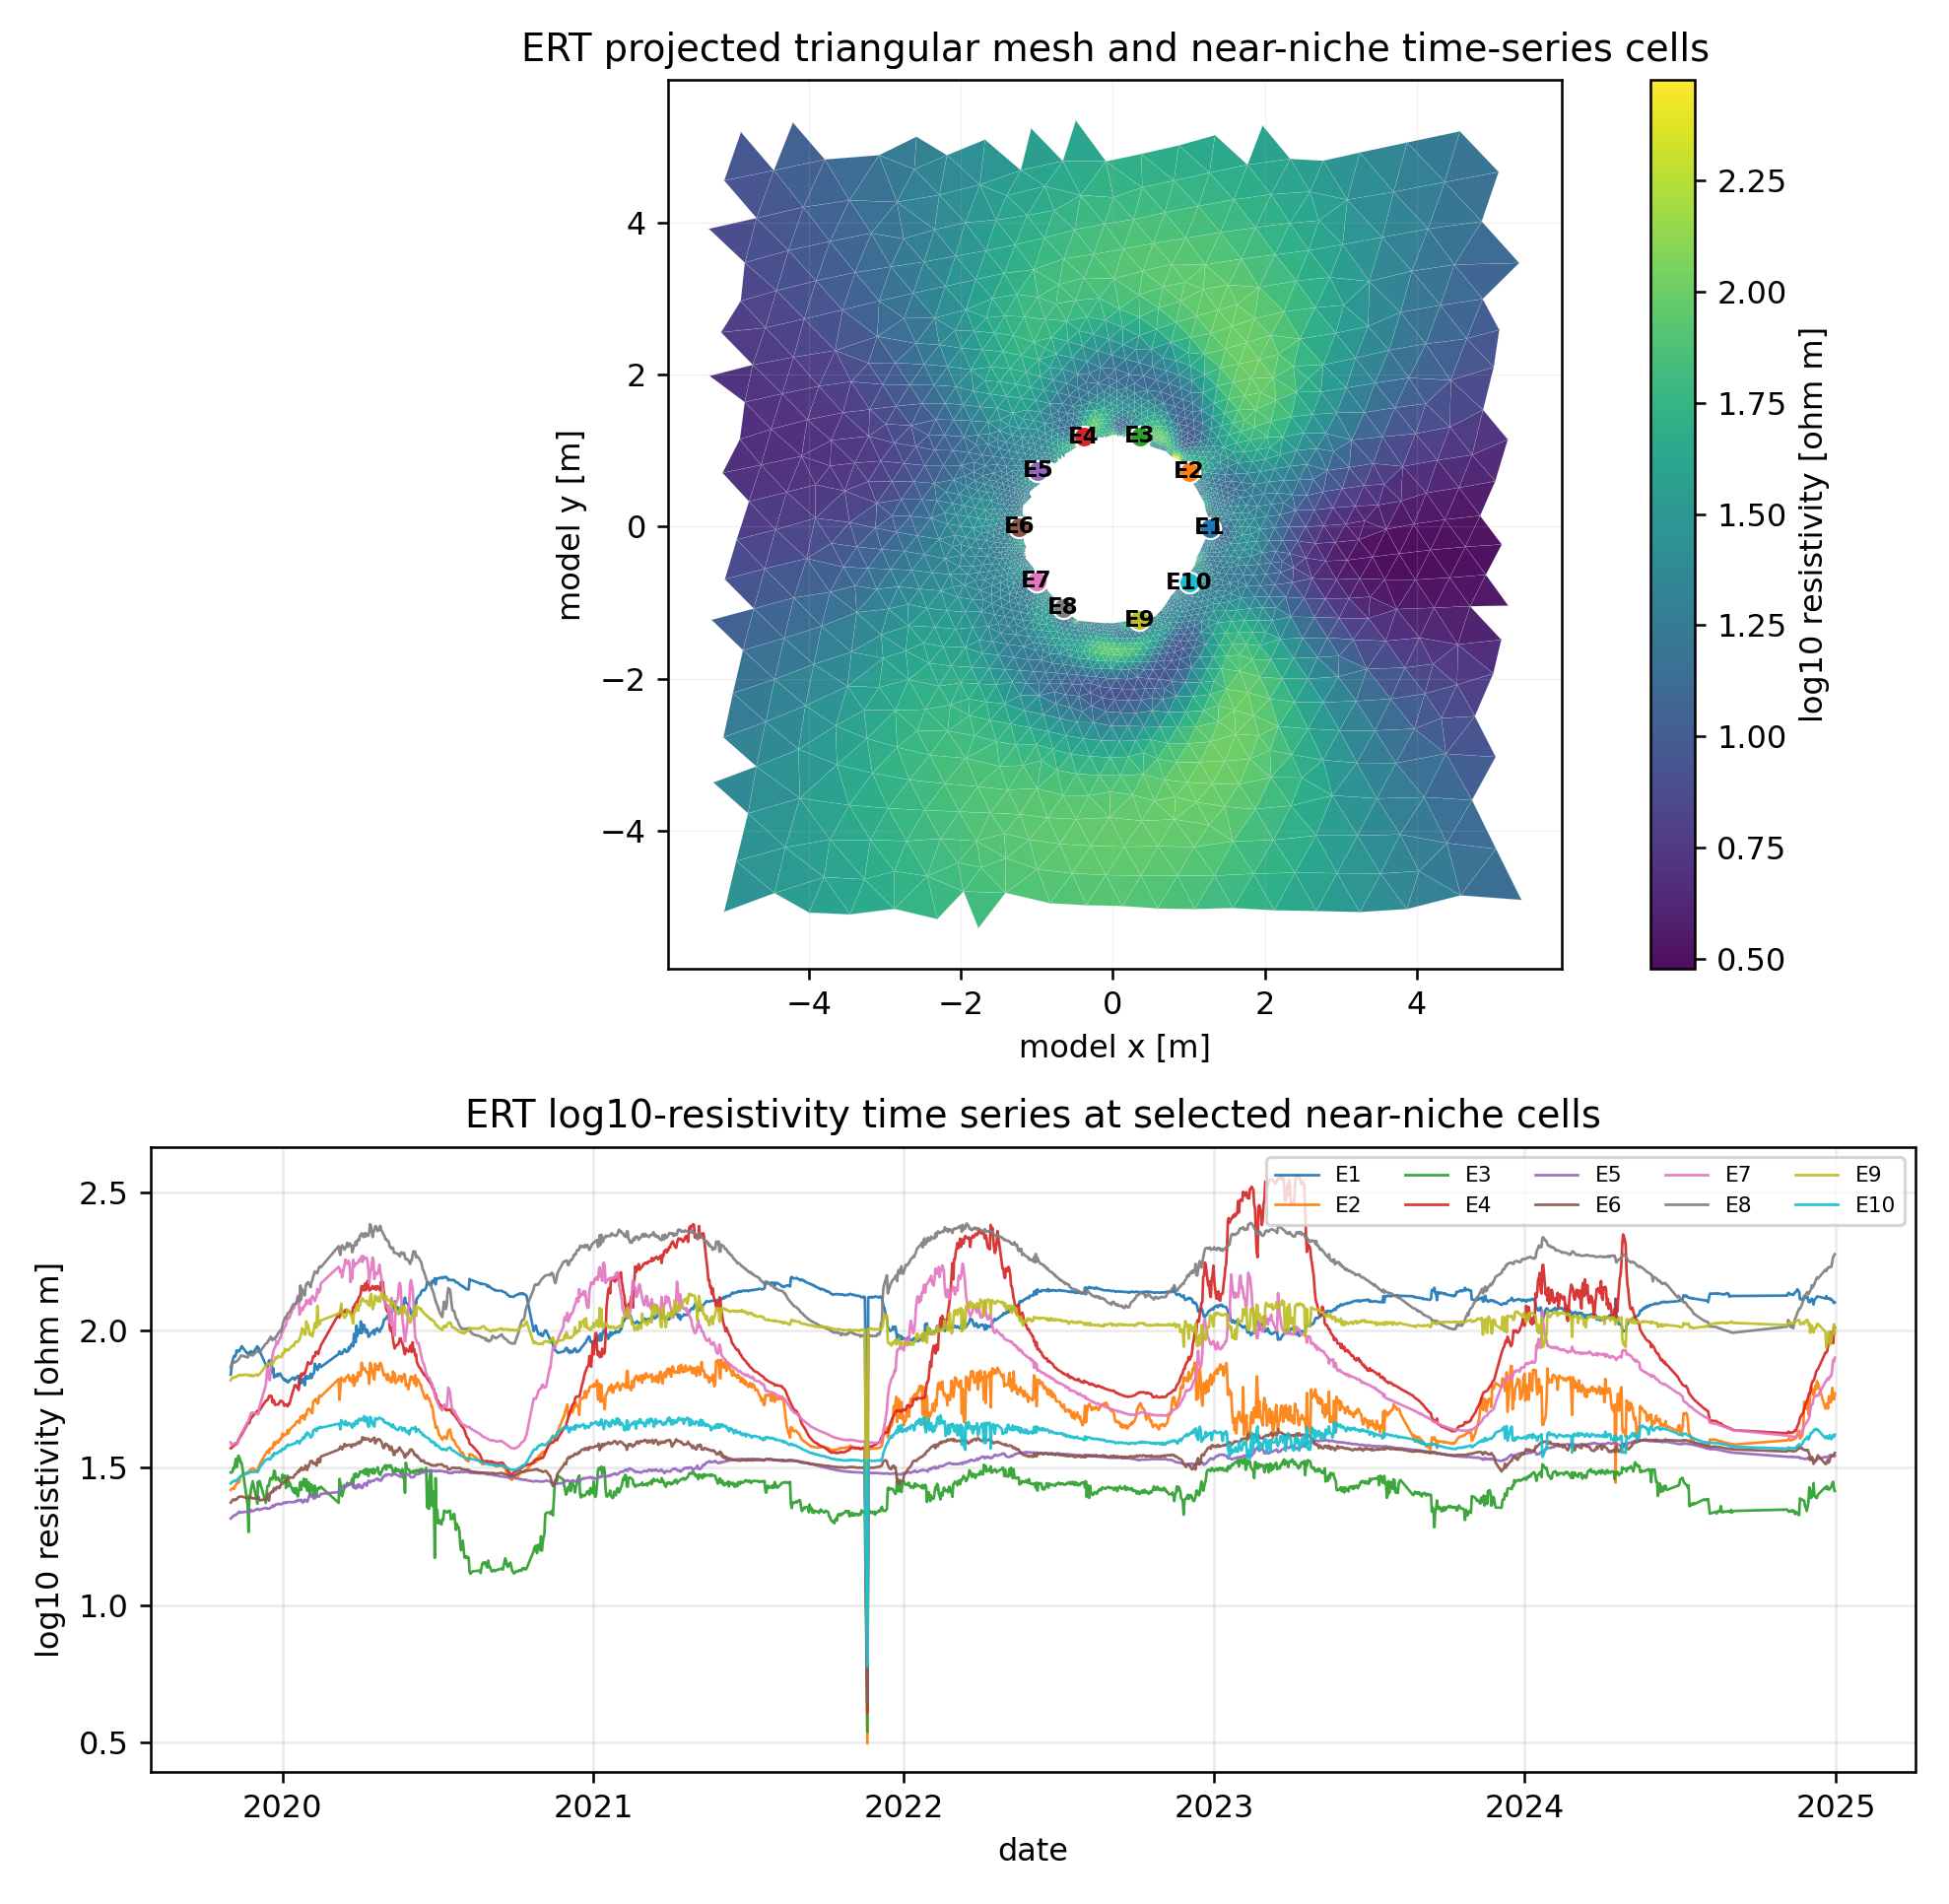
\includegraphics[width=0.98\textwidth]{resources/figures/measurement_ert_data.png}
  \caption{ERT measured-data visualisation.  The upper panel shows a projected
  reference log10-resistivity field and selected support cells; the lower panel
  shows their log10-resistivity histories over matched ERT timesteps.}
  \label{fig:ert-data}
\end{figure}

\FloatBarrier
\section{Taupe/TDR Measurements}
\label{sec:measurement-taupe}

\paragraph{Meaning.}
The Taupe/TDR workbook provides a dielectric or ARDP-derived water-content proxy.
The provided files do not yet prove whether the values are calibrated volumetric water
content, apparent relative dielectric permittivity, or another Taupe-specific proxy.
For that reason the safe current interpretation is a same-series trend diagnostic,
not an absolute saturation residual.  General TDR literature supports the link
between dielectric response and water content, but the CD-A claystone calibration
must be supplied before absolute use
\citep[Sec.~4.4]{Ziefle2024Characterization}
\citep[review and Secs.~1--2]{Robinson2003TDRReview}
\citep[Taupe/TDR technical slides]{TaupeTDREmail2026}.

\paragraph{Position in the domain.}
The source sheets A3, A4, A7, and A8 correspond to Taupe supports and EDZ distance
bands.  A3 and A4 are mapped into the current OGS frame.  A7 and A8 are kept
in the workbook and operator tables as closed-side context, but their support maps
to the \(x\approx 12\,\mathrm{m}\) side and falls outside the present open-niche
comparison.

\begin{figure}[htbp]
  \centering
  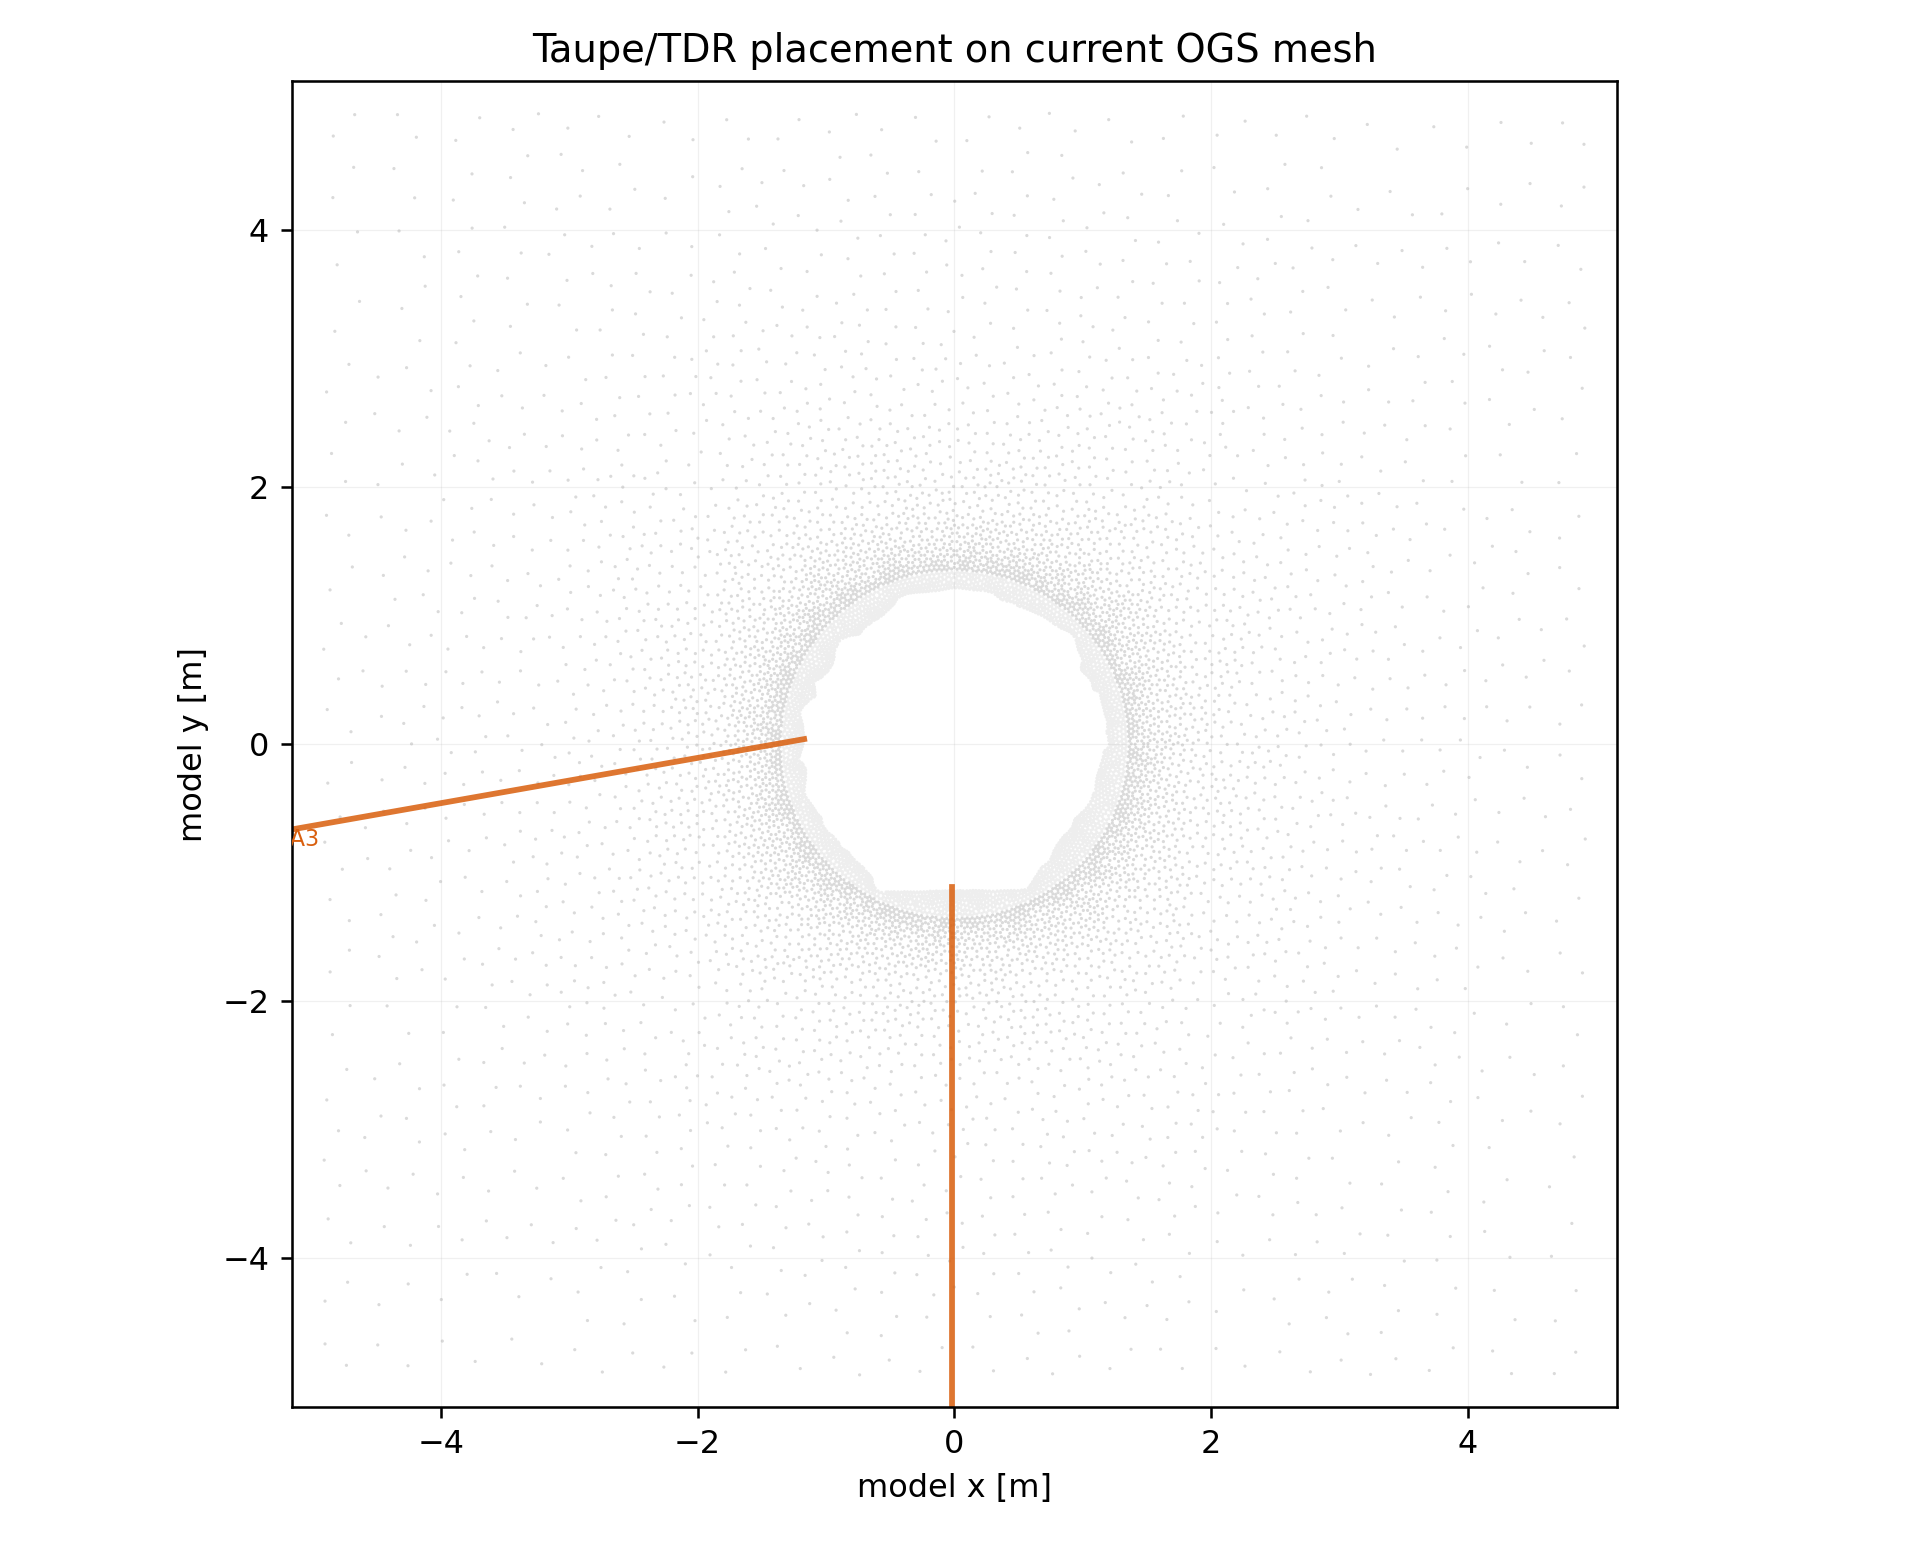
\includegraphics[width=0.86\textwidth]{resources/figures/measurement_taupe_location.png}
  \caption{Mapped Taupe/TDR line supports.  A3 and A4 are the current in-domain
  supports for trend diagnostics; A7 and A8 remain source-data context.}
  \label{fig:taupe-location}
\end{figure}

\paragraph{Time of measurement.}
The processed Taupe/TDR layer has 5088 sensor-date-band rows from 2019-12-01 to
2025-10-10.  The rows are grouped by sensor and EDZ band, including 0--10, 10--20,
20--30, 30--40, 40--50, and aggregate 0--50 cm bands from the niche wall.

\paragraph{Measured value, units, and model link.}
The workbook values span approximately 9.87 to 11.00 in source units.  Until the
unit is confirmed, the model comparison is the standardized trend
\[
  r_i^{\mathrm{Taupe}}
  :=
  H_i^{\mathrm{Taupe}}(u)
  -
  d_i^{\mathrm{Taupe}},
  \qquad
  \theta_{\mathrm{model}}=\por\Sl ,
\]
where \(H_i^{\mathrm{Taupe}}\) is the sensor/band observation operator applied to
the OGS state and \(d_i^{\mathrm{Taupe}}\) is the measured Taupe/TDR value after the
accepted baseline or calibration.  In the current diagnostic mode,
\(H_i^{\mathrm{Taupe}}\) and \(d_i^{\mathrm{Taupe}}\) are standardized within sensor
and EDZ band; if a calibration is supplied, the same support can become a
\revreplace{16}{absolute water-content or dielectric residual}{calibrated
direct-value likelihood residual in physical water-content, permittivity, or
another stated unit}{\annCommentSixteen}.  That residual informs the posterior only
after it is paired with an uncertainty, for example through
\((H_i^{\mathrm{Taupe}}(u)-d_i^{\mathrm{Taupe}})/\sigma_i^{\mathrm{Taupe}}\).

\paragraph{Uncertainty and reliability.}
The trend operator is ready as a diagnostic, but calibrated likelihood residual
weights are not.  The missing items are the workbook unit, calibration equations,
baseline convention, sensor and band uncertainties, and whether bound/interlayer
water affects the dielectric response in the same way as mobile pore water.

\subsubsection*{Current computational use.}
With the available source data now, Taupe/TDR can be used as a same-sensor,
same-band trend diagnostic for mapped A3/A4 supports.  The current operator should
band-average \(\theta_{\mathrm{model}}=\por\Sl\) over the corresponding EDZ-depth
support, subtract a series baseline, standardize within sensor and band, and compare
only the timing, sign, and relative amplitude of changes.  This avoids pretending
that the workbook unit is already an absolute volumetric water content or dielectric
permittivity.  The literature supports the general TDR water-content link, while
the Taupe stream still needs CD-A-specific calibration before absolute use
\citep[review and Secs.~1--2]{Robinson2003TDRReview}
\citep[Taupe/TDR technical slides]{TaupeTDREmail2026}
\citep[Taupe source workbook and support files]{CDAProvidedMeasurementFiles2025}.

The inverse role is indirect: Taupe/TDR can help reject permeability or boundary
candidates that produce the wrong wetting/drying trend near the EDZ.  It cannot yet
identify absolute saturation, porosity, retention, or bound-water response because
the sensor unit and calibration are still open.

\subsubsection*{Grounding questions.}
\revnote{51}{\pdfAnnComment{34}{!!!}{The Taupe workbook value remains a source-unit
gate: the paper treats it as a dielectric or water-content proxy until the unit and
calibration are confirmed.}}
\revnote{52}{\pdfAnnComment{35}{nerozumim}{The unclear phrase has been replaced by
calibrated likelihood residual, meaning a physical-unit or calibrated-unit
measurement mismatch with an observation operator and uncertainty that can enter
the posterior.}}
\revnote{53}{\pdfAnnComment{36}{nerozumim}{The weighting answer states that sensor,
cable, band, and time correlations must be grouped until covariance or
independent-noise assumptions are supplied.}}
\gqGroundingTable{tab:grounding-taupe}
{Grounding questions for Taupe/TDR measurements.}
{
\gqPair{gqGate}{Gate}{\qid{Q060} What does the Taupe workbook value represent?}{Unknown from the available source files; treat it as a source-unit dielectric/water-content proxy until
calibrated units are confirmed.}
\gqPair{gqDiagnostic}{Diagnostic}{\qid{Q061} How should Taupe/TDR be linked to OGS now?}{Compare standardized EDZ-band trends against band-averaged
\(\theta=\por\Sl\) changes for A3/A4.}
}

\begin{figure}[htbp]
  \centering
  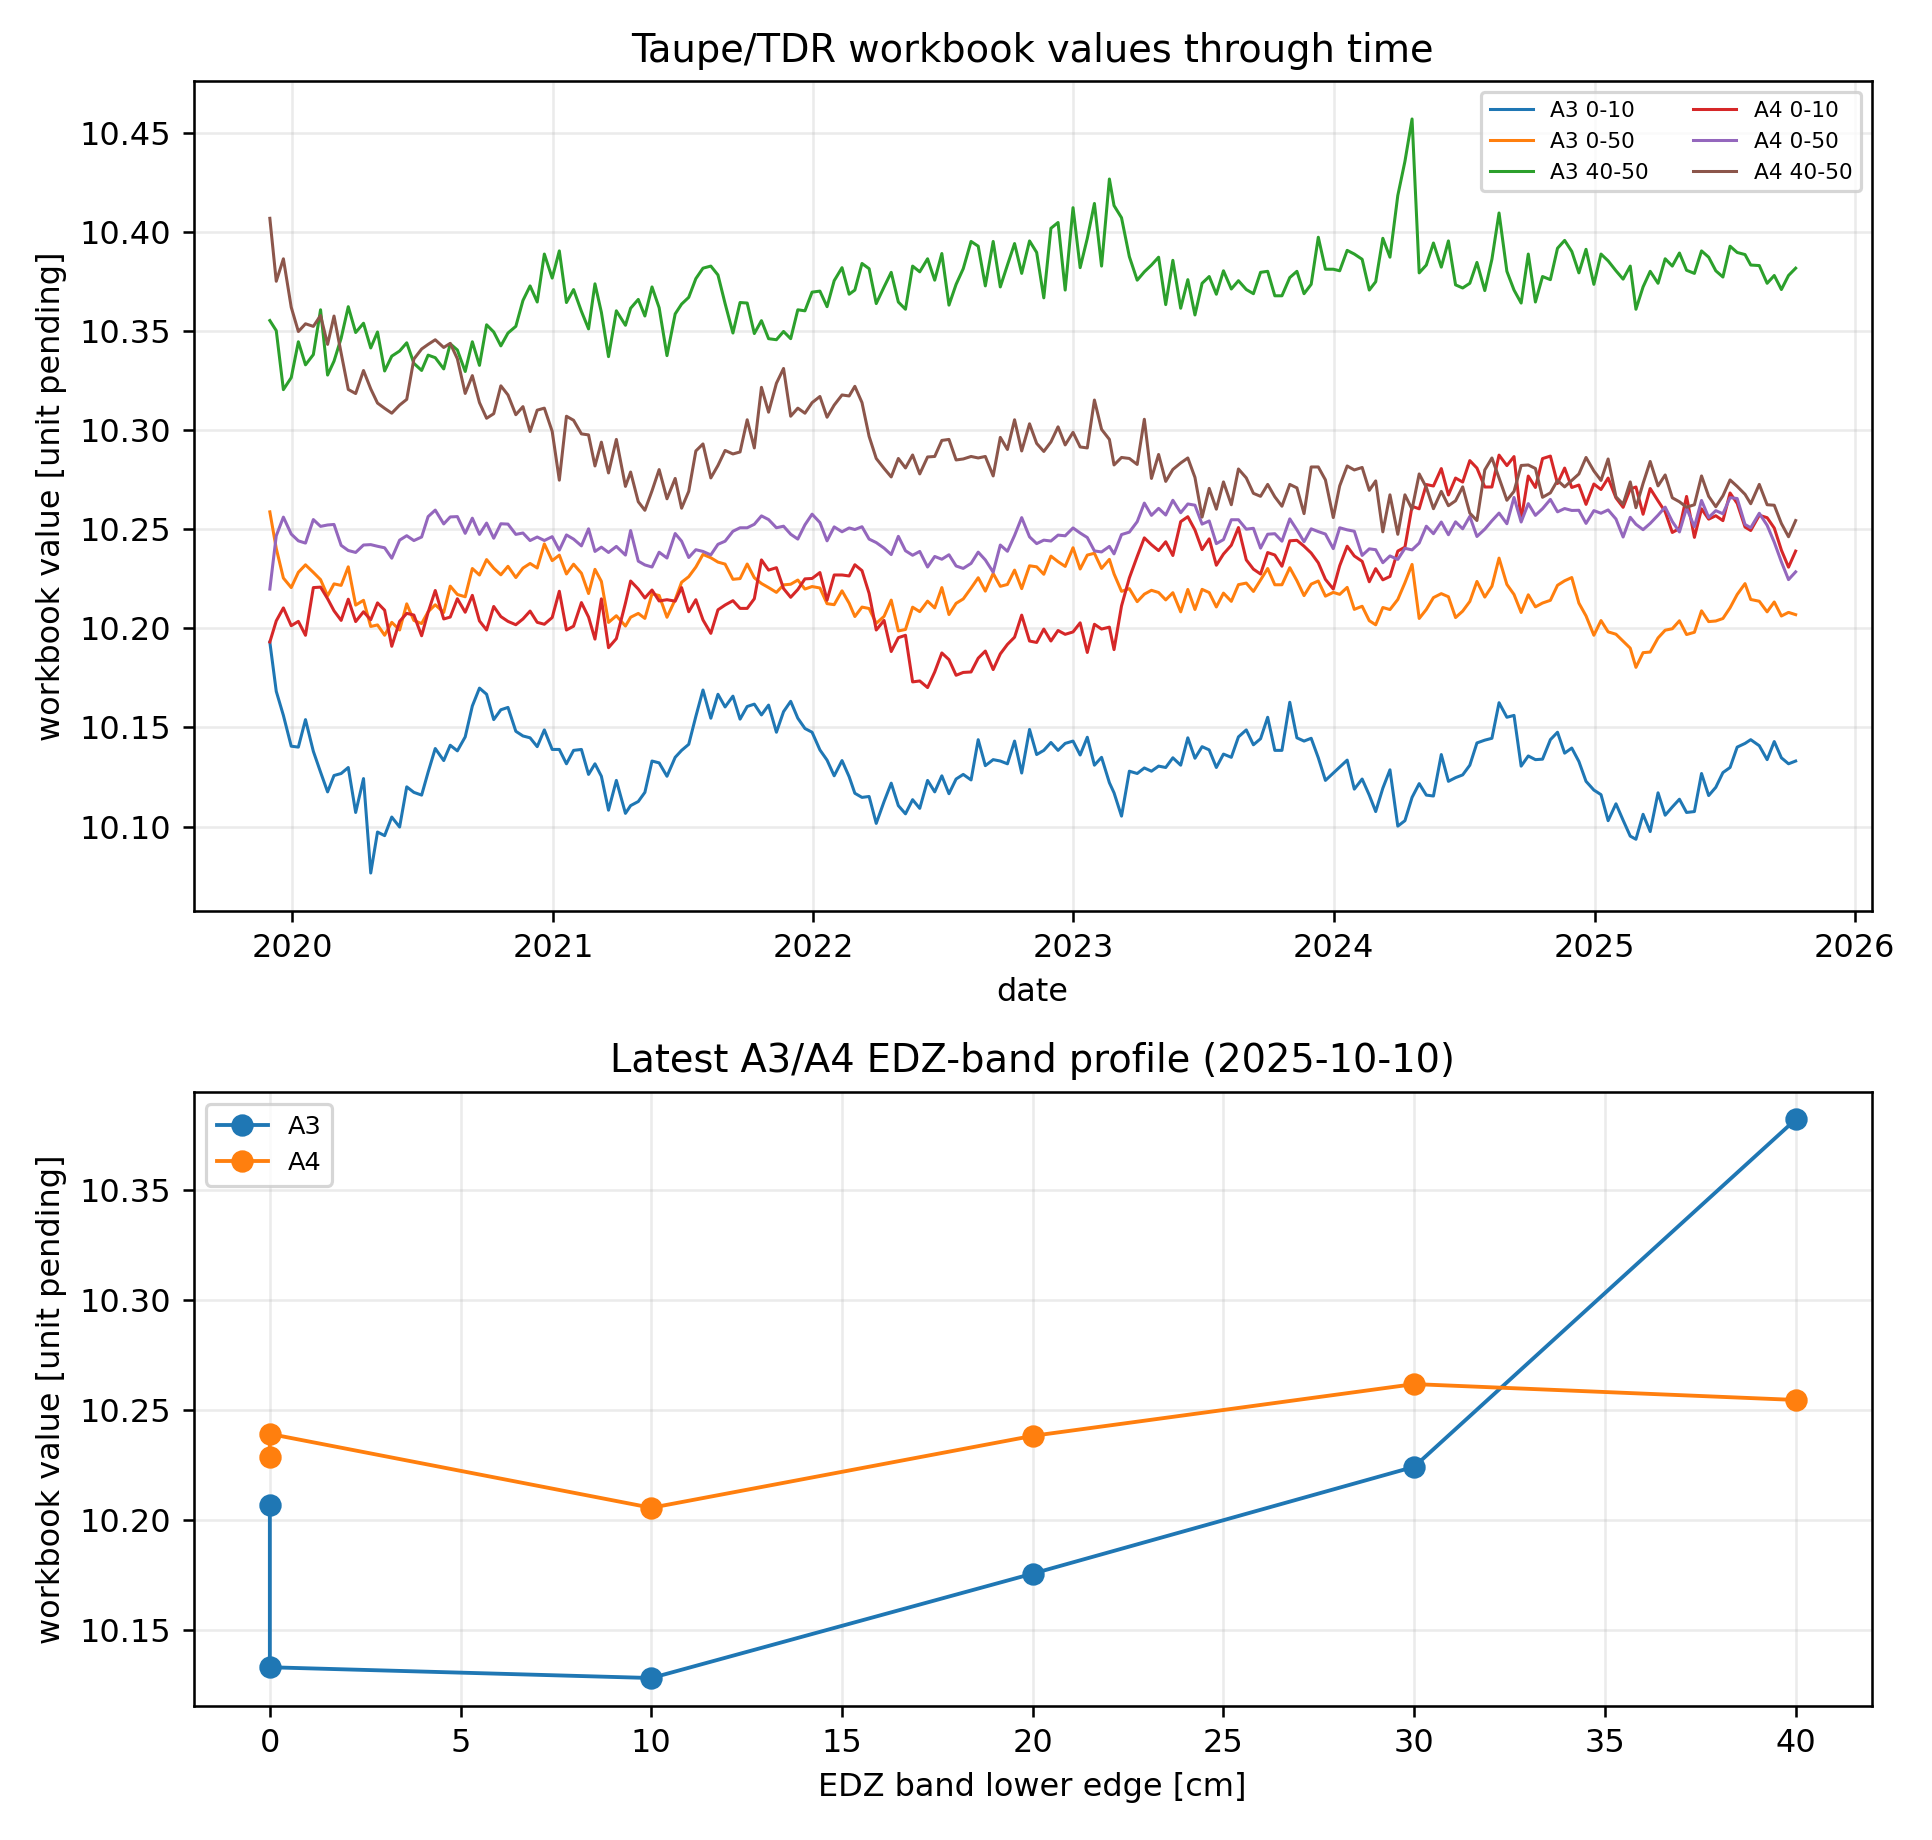
\includegraphics[width=0.98\textwidth]{resources/figures/measurement_taupe_data.png}
  \caption{Taupe/TDR measured-data visualisation.  The upper panel shows
  representative A3/A4 EDZ-band histories; the lower panel shows a latest EDZ-band
  profile.  Values are retained in source workbook units.}
  \label{fig:taupe-data}
\end{figure}

\FloatBarrier
\section{RH, Suction, and Open-Niche Pressure Forcing}
\label{sec:measurement-rh}

\paragraph{Meaning.}
The RH workbooks measure relative humidity, not liquid pressure directly.  Under a
Kelvin-equation convention, RH can be converted to a capillary-pressure or
gauge-liquid-pressure candidate.  This makes RH primarily a boundary-condition
source or check for the open niche.  It can later inform retention or boundary
uncertainty, but it is not an interior material residual.

\paragraph{Position in the domain.}
The RH/suction supports are near the open-niche boundary and are mapped as
boundary-check points in the OGS frame.  Their role is to test whether the
time-dependent boundary curve \(p_E(t)\) is consistent with humidity-derived
suction evidence.

\begin{figure}[htbp]
  \centering
  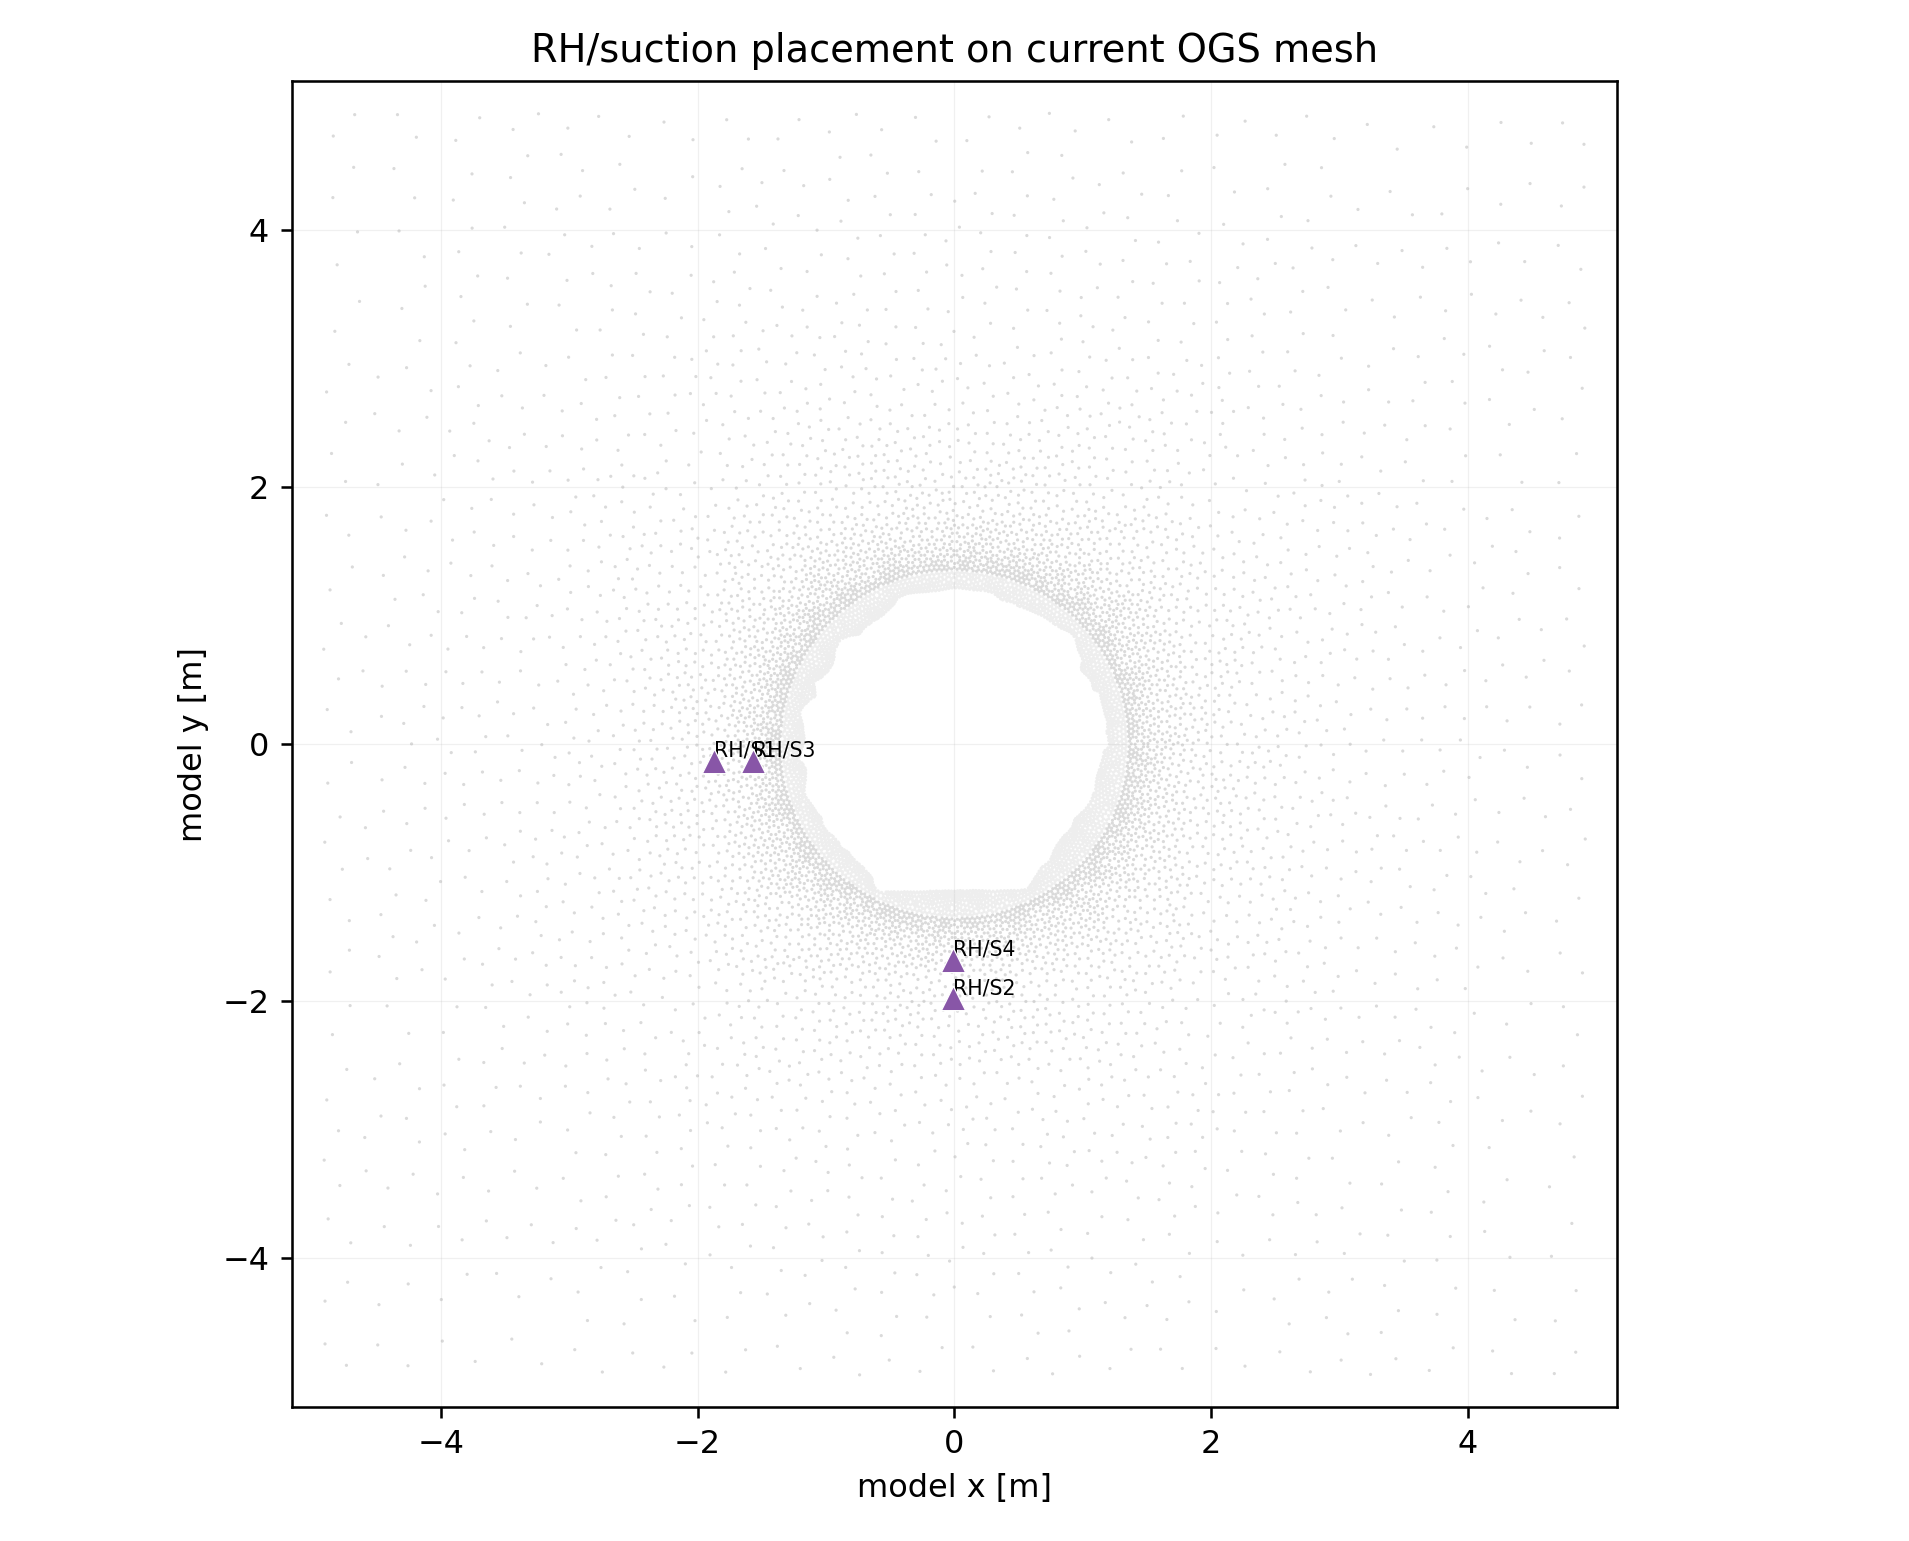
\includegraphics[width=0.86\textwidth]{resources/figures/measurement_rh_location.png}
  \caption{Mapped RH/suction support points used to check the open-niche pressure
  boundary.  These are boundary-forcing supports, not cell-wise material
  observations.}
  \label{fig:rh-location}
\end{figure}

\paragraph{Time of measurement.}
The processed RH layer contains 4247 daily rows from 2021-12-16 to 2025-09-04 for
RH5, RH6, RH7, and RH8.  RH5 and RH6 are the cleanest open-twin evidence.  RH7 and
RH8 contain low outliers near 13\% RH and require stronger screening.

\paragraph{Measured value, units, and model link.}
The source unit is RH in percent.  We convert it to a gauge-pressure candidate by
\[
  \pl^{\mathrm{Kelvin}}
  =
  \frac{\rho_lRT}{M_w}\ln(\mathrm{RH}),
\]
where RH is a fraction, \(T=298.15\,\mathrm{K}\), and
\(\rho_l=1095\,\mathrm{kg\,m^{-3}}\).  The constants \(R\) and \(M_w\) are the molar
gas constant and molar mass of water used by the Kelvin conversion.  Since
\(\ln(\mathrm{RH})<0\), the converted liquid pressure is negative in the same
suction convention used by the active
open-niche curve.  This is consistent with \(p_c=-\pl\) in the Richards model
\citep[pp.~448--452]{Thomson1871Kelvin}
\citep[Sec.~3, Eqs.~1--2]{WaterContentEDZ2024}.

\paragraph{Uncertainty and reliability.}
The active OGS curve has 845 rows and spans approximately \(-53.24\) to
\(-5.23\,\mathrm{MPa}\).  The RH boundary check compares 2280 rows inside the active curve
time range and finds large differences between RH-derived pressure candidates and
the active curve.  Therefore \(p_E(t)\) should remain an existing OGS input, not a
verified RH-derived forcing, until the source sensors, filtering, smoothing, time
origin, interpolation, and extension policy are reconstructed.

\subsubsection*{Current computational use.}
With the available source data now, RH/suction should be used as boundary-forcing
provenance and uncertainty information for the open-niche pressure curve, not as an
independent interior residual.  The current best transfer is to convert screened RH
records to a Kelvin pressure candidate with the stated constants, compare that
candidate to the active XML curve \(p_E(t)\), and represent the mismatch as a
boundary-condition gate or scenario envelope.  This is grounded in the active curve
values, RH workbook check, and the CD-A water-content/RH formulation where negative
liquid pressure represents suction through the chosen pressure convention
\citep[pp.~448--452]{Thomson1871Kelvin}
\citep[Sec.~3, Eqs.~1--2]{WaterContentEDZ2024}
\citep[RH source workbooks used for the generated boundary checks]{CDAProvidedMeasurementFiles2025}.

In the inverse problem, uncertain \(p_E(t)\) is dangerous because permeability,
retention, and boundary suction all control similar drying/wetting transients.
If the boundary curve is treated as exact while its provenance is unresolved, the
fit can falsely compensate by changing \(\KK(\xx)\) or retention parameters.

\subsubsection*{Grounding questions.}
\revnote{54}{\pdfAnnComment{37}{jasne}{The RH table keeps RH as an input-side
boundary source or check for \(p_E(t)\), not as an interior output residual.}}
\revnote{55}{\pdfAnnComment{38}{chceme ujasnit vztah}{The RH-to-pressure relation is
stated through the Kelvin equation with RH fraction, temperature, density, gas
constant, molar mass, and \(p_c=-\pl\).}}
\revnote{56}{\pdfAnnComment{39}{chceme ujasnit?}{Negative model pressure is defined
as liquid pressure relative to the gas/reference pressure; with \(p_c=-\pl\), it is
positive suction.}}
\revnote{57}{\pdfAnnComment{40}{spise bych se ptal na nejpouzitelnejsi sensor}{The
table answers this as a sensor-selection gate: RH5/RH6 are the cleanest current
open-niche candidates, but filtering, outlier handling, and time alignment remain
open.}}
\gqGroundingTable{tab:grounding-rh}
{Grounding questions for RH/suction and pressure-boundary forcing.}
{
\gqPair{gqGate}{Gate}{\qid{Q067} Which sensors define the open-niche boundary?}{RH5/RH6 are the cleanest source candidates, but final use needs explicit sensor
selection, filtering, high-RH/low-outlier handling, and time alignment.}
\gqPair{gqGate}{Gate}{\qid{Q087} Can we obtain the full RH/suction source data from the start of the active \(p_E(t)\) curve?}{Request
the complete source data behind the open-niche pressure forcing from its 2019 start:
raw RH, temperature, suction or processed-pressure rows, sensor ids, timestamps,
screening flags, and the script or table that converts those values into
\(p_E(t)\).  The key provenance question is whether the initial \(p_E\) segment in
the XML was derived from these measurements, manually prescribed, or extended by a
separate preprocessing rule.}
\gqPair{gqGate}{Gate}{\qid{Q069} What would fully ground the pressure boundary?}{Source table, sensor selection, smoothing/filtering, interpolation and
extrapolation rules, calendar time origin, sign/unit convention, and a covariance
or scenario envelope for boundary uncertainty.}
}

\begin{figure}[htbp]
  \centering
  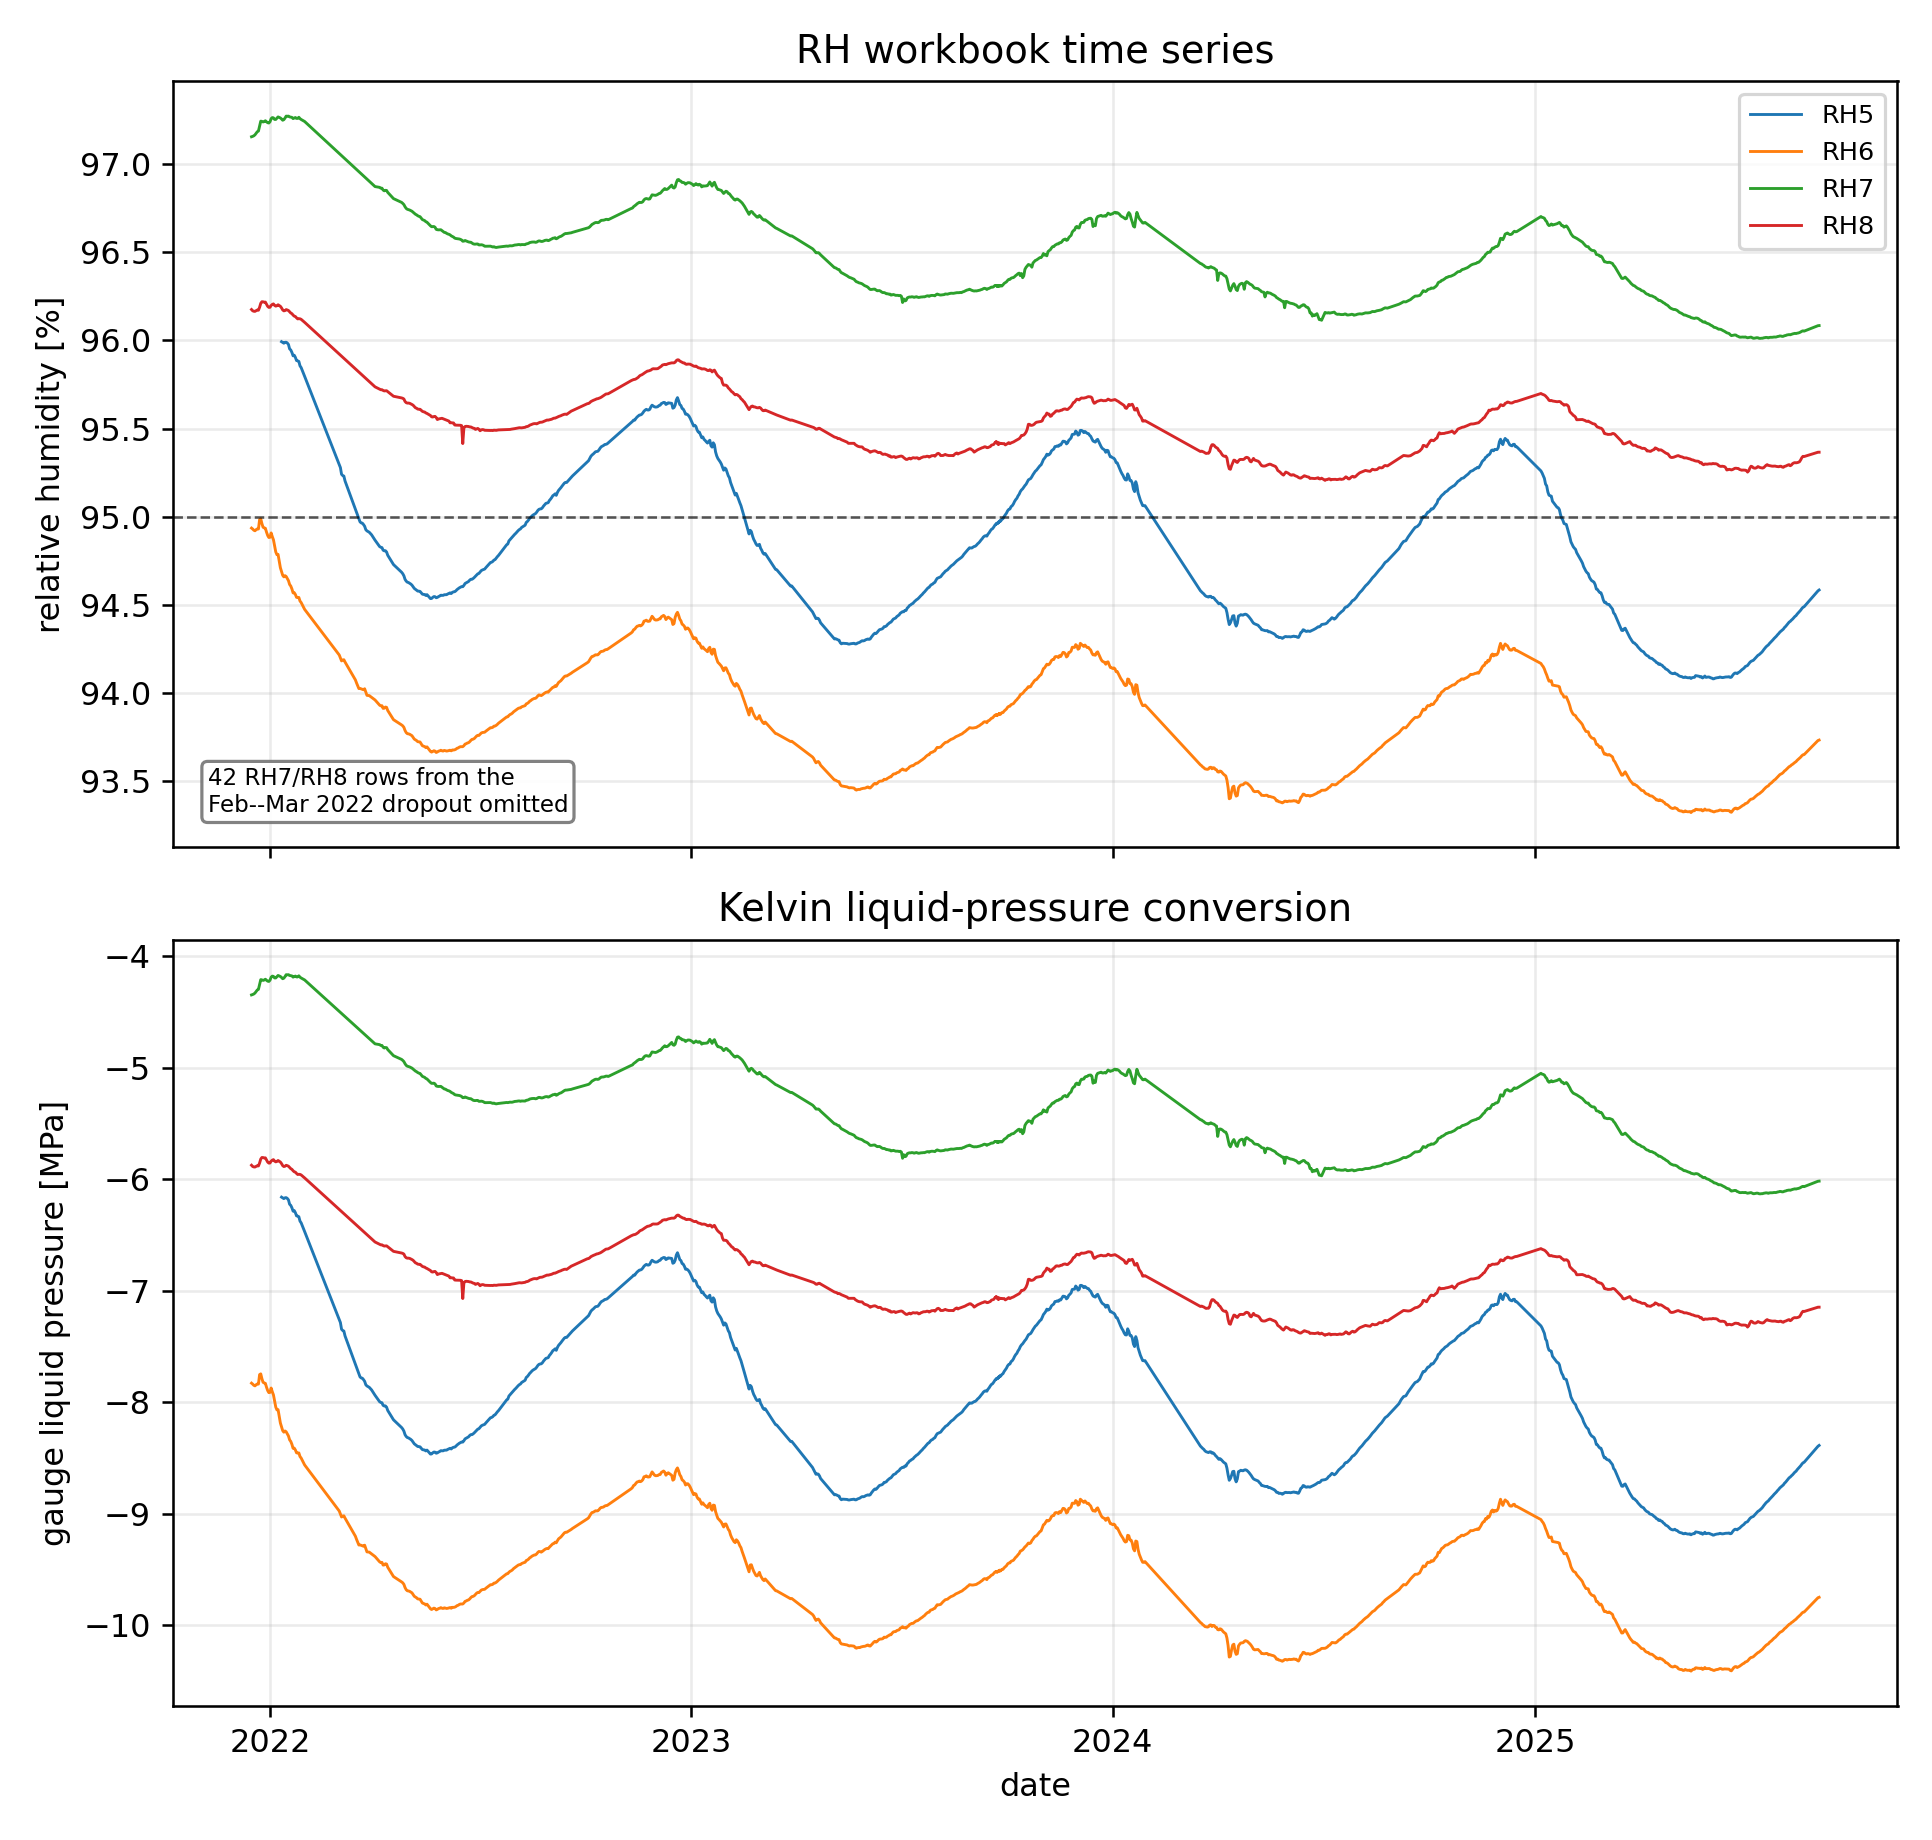
\includegraphics[width=0.98\textwidth]{resources/figures/measurement_rh_data.png}
  \caption{RH and Kelvin-converted pressure visualisation.  The upper panel shows
  RH5--RH8 histories after omitting the flagged RH7/RH8 dropout interval; the lower
  panel shows the corresponding gauge liquid-pressure conversion in MPa.}
  \label{fig:rh-data}
\end{figure}

\FloatBarrier
\section{Direct Pressure Measurements}
\label{sec:measurement-pressure}

\paragraph{Meaning.}
The direct-pressure stream is the mini-piezometer stream.  In the CD-A
measurement inventory, mini-piezometers measure pore pressure with unit Pa
\citep[Table~1]{Ziefle2024Characterization}.  The VEIS paper confirms that CD-A
has borehole sensors for pressure measured by minipiezometers and that sensor
databases store sensor names, date/time stamps, and measured values
\citep[Secs.~2.4 and 3.2]{Graebling2022VEIS}.  The 2026 email-provided technical
discussion identifies BCD-A28 to BCD-A31 as the current mini-piezometer set and
shows their pressure trends in kPa \citep[PDF p.~32]{CDATDSlides2026Email}.

\paragraph{Position in the domain.}
Figure~\ref{fig:pressure-minipiezometer-trends} includes the source-slide
location inset for A28--A31.  That inset is enough to identify the instrument
family and open/closed-twin context, but it is not yet an accepted OGS point set.
A usable pressure residual still needs individual sensor coordinates or trace
supports, sensor elevations/depths, and a rule for projecting each 3D sensor
support to the present 2D slice.

\begin{figure}[htbp]
  \centering
  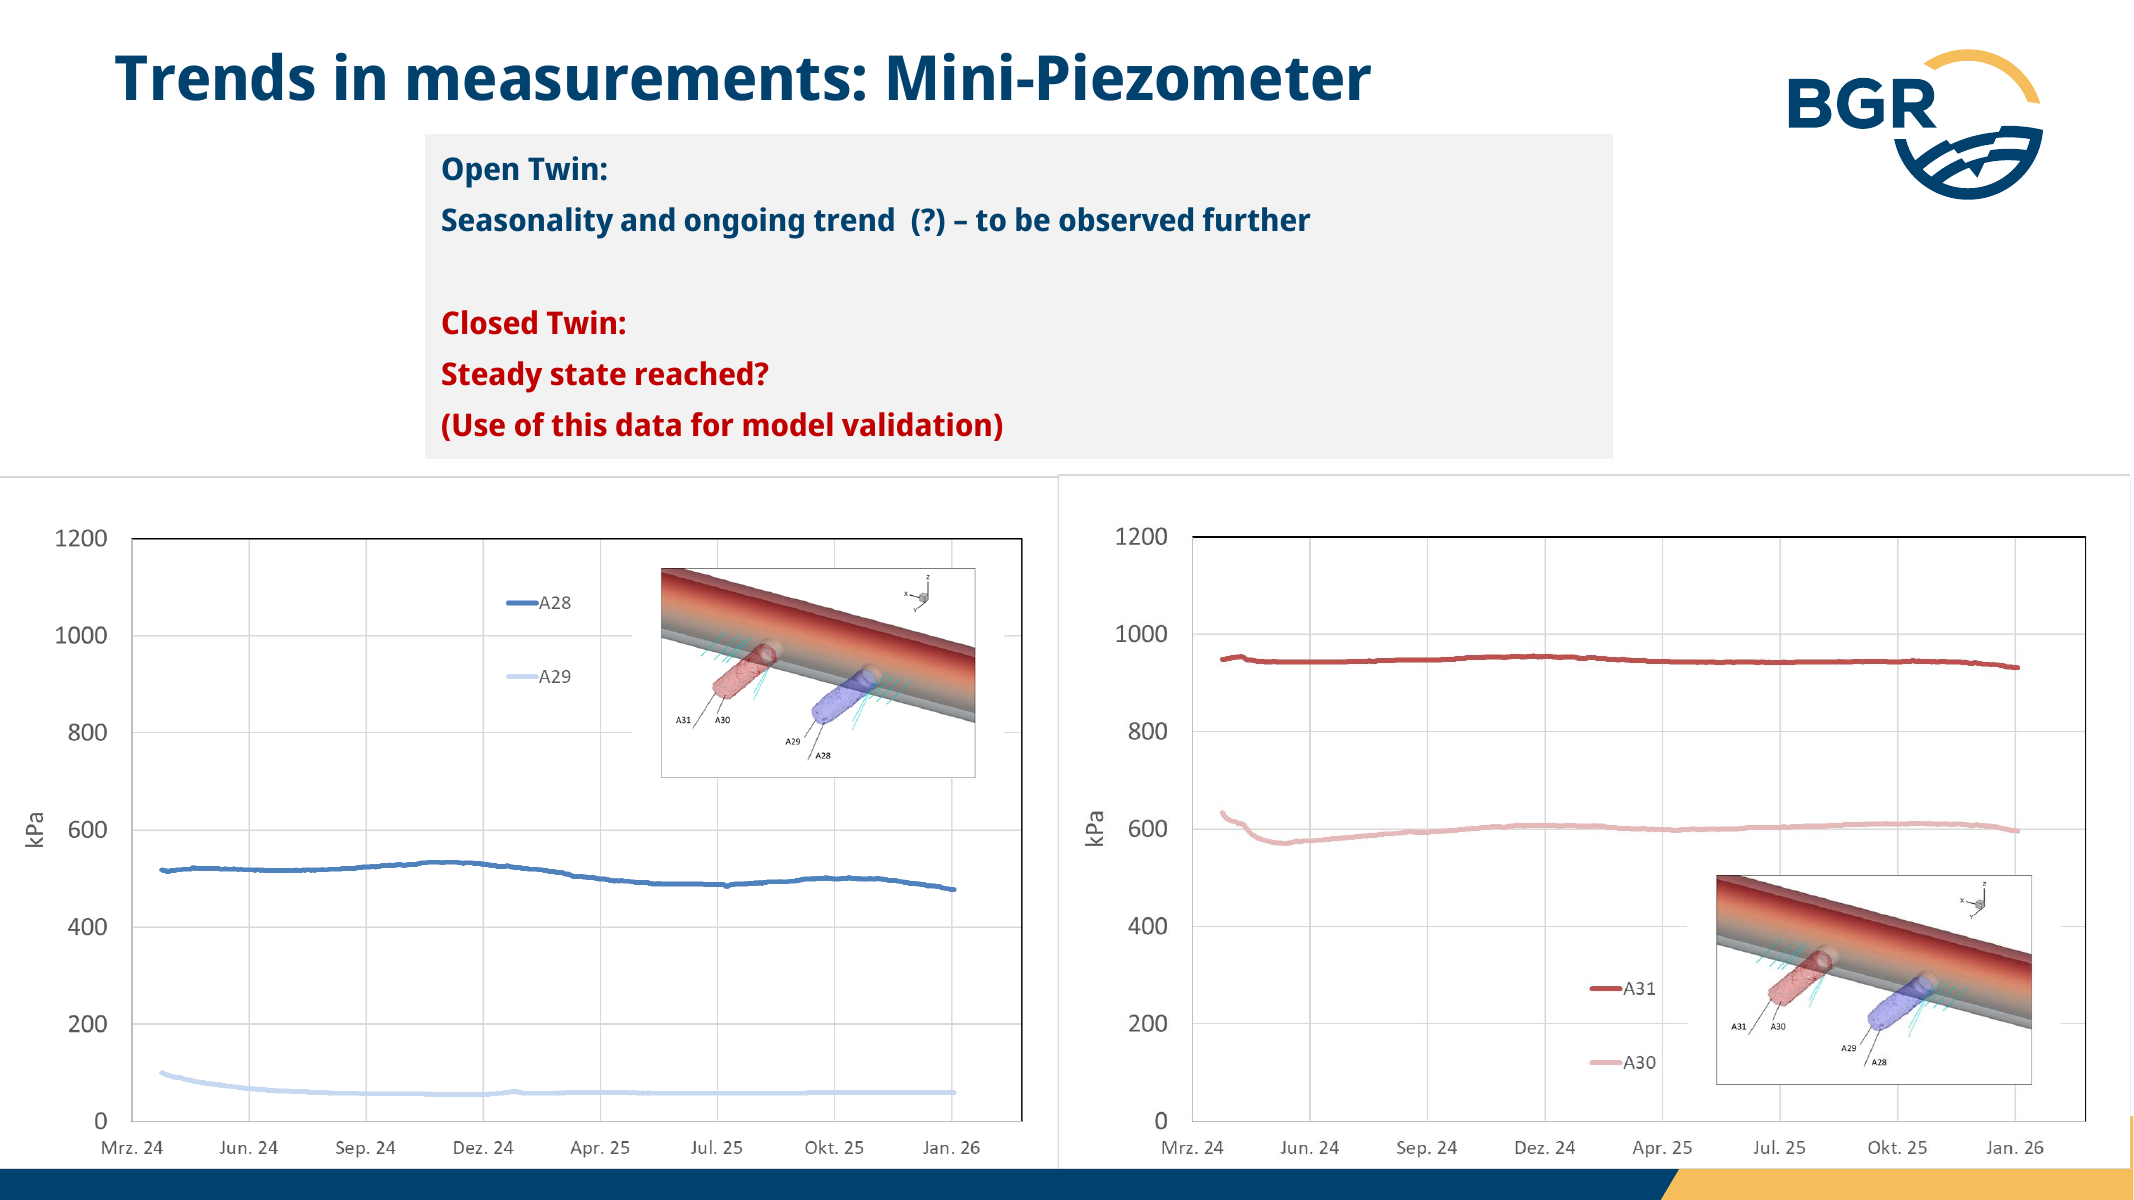
\includegraphics[width=\textwidth]{resources/figures/measurement_pressure_minipiezometer_trends.png}
  \caption{Mini-piezometer trend evidence from the 2026 technical discussion
  slides.  The plotted values are in kPa and cover approximately March 2024 to
  January 2026.  The open twin shows seasonality and an ongoing trend; the closed
  twin is shown only as source context for this open-niche note.  This is a
  source-slide plot, not a machine-readable export or current residual.}
  \label{fig:pressure-minipiezometer-trends}
\end{figure}

\paragraph{Time of measurement.}
The source plot spans about March 2024 to January 2026.  The May 2026 minutes
state that BCD-A28 to BCD-A31 were working well, and list pore-pressure
measurements as later comparison targets for the modelling workflow
\citep[PDF p.~4 and p.~8]{CDATDMinutes2026Email}.  The sampled numeric export behind
the plot is still absent from the current provided catalogue, so exact timestamps,
sampling interval, maintenance gaps, and quality flags remain unavailable.

\paragraph{Measured value, units, and model link.}
The source plot uses kPa.  The public CD-A inventory names the quantity as pore
pressure in Pa, but the provided export must still state whether the stored values
are absolute pressure, gauge pressure, hydraulic head, or another Geoscope
conversion.  Once that reference convention is known, the model link is direct:
sample \(\pl(\xx,t)\) at the sensor support and convert pressure unit, elevation
head, atmospheric reference, and sensor depth consistently with the model pressure
convention.

\paragraph{Uncertainty and reliability.}
This stream is promising but not residual-ready.  The required export must include
timestamps, units, sensor ids, coordinates or support ids, zero/reference
convention, calibration, temperature compensation, quality flags,
maintenance/failure flags, and raw-file provenance.  The 2D model error may be
significant if a mini-piezometer samples a local 3D feature or lies outside the
effective support of the modeled slice.

\subsubsection*{Current computational use.}
With the available source data now, direct pressure measurements are a blocked but
high-value future residual.  The source-slide trends prove that the stream exists
and has physically meaningful evolution, but the paper does not yet have the
machine-readable export needed for fitting.  Once that export is available, the
operator should be a direct sample or support average of OGS \(\pl(\xx,t)\), or a
hydraulic-head comparison after elevation and reference-pressure conversion.  This
would directly test whether the far-field pressure, open-niche boundary curve,
initial pressure field, and fitted permeability field are mutually consistent
\citep[Table~1]{Ziefle2024Characterization}
\citep[Secs.~2.4 and 3.2]{Graebling2022VEIS}
\citep[PDF p.~32]{CDATDSlides2026Email}
\citep[provided pressure/HM source files and generated trend figures]{CDAProvidedMeasurementFiles2025}.

The most important current modelling use is not to fit the slide image.  It is to
request the pressure export in a form that closes the pressure-reference ambiguity.
Confusing absolute pressure, gauge pressure, hydraulic head, suction, or capillary
pressure would shift the residual and can force incorrect changes in boundary
pressure, initial pressure, or \(\KK(\xx)\).

\subsubsection*{Grounding questions.}
\revnote{58}{\pdfAnnComment{41}{prakticky chceme vedet, jak interpretovat
data(2D/3D)?}{The pressure section marks this as a 2D comparison gate: each sensor
needs coordinates, elevation/depth, support, and a defensible 3D-to-2D projection
before it becomes a pressure residual.}}
\gqGroundingTable{tab:grounding-pressure}
{Grounding questions for direct pressure measurements.}
{
\gqPair{gqBlocked}{Blocked}{\qid{Q070} Do direct pore-pressure measurements exist for this model?}{Yes as a documented mini-piezometer stream and source-slide trend; no
residual-ready numeric export is present yet.}
\gqPair{gqGate}{Gate}{\qid{Q071} How should pressure be linked to OGS?}{Compare to \(\pl(\xx,t)\) or hydraulic head only after units, elevation,
absolute/gauge/reference convention, and sensor support are known.}
\gqPair{gqGate}{Gate}{\qid{Q073} What 2D-model caveat is needed?}{Each sensor may sample a 3D hydraulic path or feature outside the modeled slice;
the export must support a defensible 3D-to-2D comparison rule.}
\gqPair{gqGate}{Gate}{\qid{Q088} Can we obtain the exact data and positions for BCD-A28--A31?}{Request the machine-readable mini-piezometer time series together with exact
sensor positions: coordinates in the source frame, borehole or screened interval,
elevation/depth, open- or closed-twin assignment, timestamps, raw pressure units,
pressure reference, calibration and maintenance flags, and the accepted
3D-to-2D projection for the current OGS slice.}
}

\FloatBarrier
\section{Faults, Fractures, and Crack Geometry}
\label{sec:measurement-faults}

\paragraph{Meaning.}
This section is about large faults, fault zones, and mapped fracture geometry, not
about crackmeter time series.  The public CD-A characterization paper reports
fault planes parallel to bedding as well as non-bedding-parallel fault planes, and
summarizes the structural geology near the twin niches in its Fig.~4
\citep[Sec.~3 and Fig.~4]{Ziefle2024Characterization}.  For the OGS workflow,
these features are not observations of pressure or displacement by themselves.
They are structural information that can affect permeability, porosity, EDZ
extent, anisotropy, or prior covariance.

\paragraph{Position in the domain.}
The provided Tecplot layout contains 22 \texttt{Kluft} fracture/crack-geometry zones.
Those zones document source-frame structural supports, but they do not yet define
which 3D features intersect the current 2D model slice, what effective width should
be used, or whether the feature should become a hard material input, a prior, a
mask, or a qualitative caveat.  The email-provided HERMES input note also states that
geological characterization of fractured zones is available for CD-A
\citep[PDF p.~5]{HermesInput2024Email}.

\paragraph{Time of measurement.}
The geometry is structural, not a complete time series.  A feature can still be
used as time-dependent modelling information only if there is measured aperture,
displacement, hydraulic effect, or dated structural evolution.  Without that, it
should be treated as static structural context or as a scenario/prior field.

\paragraph{Measured value, units, and model link.}
For large faults and fracture zones, the model-facing quantities are 3D
coordinates, plane or zone geometry, width/support, aperture or hydraulic effect,
and a projection policy.  The model link is indirect: a fault may modify
\(\KK(\xx)\), \(\por(\xx)\), EDZ classification, permeability-tensor orientation,
or the prior covariance of those fields.  It is not a residual against an OGS
output unless a measured quantity, unit, time, and observation operator are
defined.

\paragraph{Uncertainty and reliability.}
The main risk is overfitting a two-dimensional permeability field to a
three-dimensional unresolved structure.  A fault or crack should become a hard input
only after the projection policy is explicit: which 3D feature intersects the 2D
slice, what width/support is assigned, whether it changes \(\KK\), \(\por\), EDZ
classification, or only the prior covariance, and which uncertainty represents
projection error.

\subsubsection*{Current computational use.}
With the available source data now, large faults and fracture geometry should enter
as structural priors, masks, or scenario definitions rather than residuals.  The
provided \texttt{.dat}/Tecplot geometry gives source-frame structural zones, and the
public CD-A characterization supports the relevance of faults and fractured zones,
but geometry alone does not define hydraulic aperture, permeability contrast, or a
time-dependent material change.  The best current use is to construct alternative
2D projection scenarios: no fault effect, a projected EDZ/fault mask, a local
permeability-basis support, or a covariance modifier for \(\KK\) and possibly
\(\por\) or tensor orientation
\citep[Sec.~3 and Fig.~4]{Ziefle2024Characterization}
\citep[PDF p.~5]{HermesInput2024Email}
\citep[geometry source file \texttt{VisualisationCDA.dat}]{CDAProvidedMeasurementFiles2025}.

For inversion, the key discipline is not to turn fault geometry into a fake
measurement.  A fault can guide where material fields are allowed to vary.  It
becomes a residual only if a numeric aperture, displacement, pressure response, or
other measured value is supplied with units, time, support, and an observation
operator.

\subsubsection*{Grounding questions.}
\revnote{59}{\pdfAnnComment{42}{Asi chceme jen navrhnout, ze budeme pracovat s
trhlinami jako extra nahodnym polem/domenou a nechat si to schvalit?}{The faults
section now proposes exactly this as current use: projected structural priors,
scenario masks, permeability-basis supports, or covariance modifiers, not hard
residuals without measured aperture or hydraulic effect.}}
\gqGroundingTable{tab:grounding-faults}
{Grounding questions for large faults and fracture geometry.}
{
\gqPair{gqDiagnostic}{Diagnostic}{\qid{Q075} What does the large-fault source measure?}{Currently it is structural geometry; no accepted residual-ready aperture,
displacement, or hydraulic-effect table is present.}
\gqPair{gqPolicy}{Policy}{\qid{Q076} How should faults link to OGS now?}{As projected structural priors, EDZ/fault masks, permeability-basis supports,
tensor-orientation context, or scenario fields.}
\gqPair{gqGate}{Gate}{\qid{Q077} Can a fault modify permeability or porosity?}{Yes as a scenario or prior, but hard modification needs independent evidence from
permeability, ERT, pressure, NMR/Taupe trends, or crack/HM data.}
\gqPair{gqGate}{Gate}{\qid{Q078} How should 3D geometry be reduced to the 2D slice?}{By an explicit intersection, influence-band, or nearest-distance projection with
effective width and uncertainty; otherwise it remains a caveat.}
\gqPair{gqGate}{Gate}{\qid{Q079} What would fully ground quantitative fault use?}{Exact source file, coordinates and units, feature identities, 3D-to-2D projection,
width/support, target fields \((\KK,\por,\mathrm{EDZ})\), time-dependence
assumption, and independent hydraulic or mechanical evidence.}
}

\FloatBarrier
\section{Geoscope, Crackometer, and Other HM Monitoring}
\label{sec:measurement-other-hm}

\paragraph{Meaning.}
The other-HM package covers measurements that can constrain mechanics, pressure,
swelling, permeability plausibility, or boundary disturbances: extensometers,
crackmeters, laser scans, miniprisma geodesy, convergence points, precision
levelling, evapometer or climate context, and Geoscope auxiliary streams.  The CD-A
inventory identifies extensometers and convergence as displacement measurements,
laser scans as niche-profile displacement measurements in micrometres, and
mini-piezometers as pore pressure measurements \citep[Table~1]{Ziefle2024Characterization}.
The email-provided HERMES input note frames the same bundle as long-term deformation,
humidity, water-content, pore-water-pressure, crack-width, piezometer,
extensometer, ERT, TDR, and laser-scan measurements \citep[PDF p.~5]{HermesInput2024Email}.

\paragraph{Position in the domain.}
The source layout contains support geometry for several HM streams, but the generic
support plots are not useful paper figures because they do not show measured
values, timestamps, units, or OGS-ready support.  Table~\ref{tab:other-hm-status}
therefore records the useful status directly.  Before fitting, each stream needs a
mapping from source frame to the current 2D model frame and, where relevant, a
3D-to-2D comparison rule.

\Needspace{32\baselineskip}
\begin{center}
\centering
\footnotesize
\renewcommand{\arraystretch}{1.12}
\captionof{table}{Other-HM measurement status in the current source catalogue.}
\label{tab:other-hm-status}
\begin{tabular}{@{}L{0.18\textwidth} L{0.25\textwidth} L{0.24\textwidth} L{0.23\textwidth}@{}}
\toprule
Stream & What it measures & Current source evidence & Model link and status\\
\midrule
Extensometer & Displacement or strain along instrument geometry. &
Geoscope/minutes evidence; BCD-A9/B10 closed-niche failure since September 2025. &
\(\uu\) or strain diagnostic; hard residual blocked until time series, geometry,
sign, and quality flags are supplied.\\
Crackmeter & Crack aperture or local relative displacement. &
Source trend plot and minutes: one closed-twin trend and open-twin seasonal
variation. &
\(\uu\), strain, or crack-aperture diagnostic; residual blocked until positions,
zero date, sign convention, units, and uncertainty are supplied.\\
Laser scans & Registered niche-surface displacement or scan-difference fields. &
Minutes state a 2026-04-20 statistical laser-scan update was sent; the provided catalogue
has only surface geometry. &
Surface-displacement diagnostic; blocked until registered products, masks,
reference epochs, and registration uncertainty are supplied.\\
Levelling & Vertical displacement at survey points. &
A small slide-summary set of height differences from the 2022-08-29/30 reference
to the 2026-03 campaign. &
Vertical \(\uu\) validation target; diagnostic only until full survey table,
coordinates, reference frame, and covariance are supplied.\\
Auxiliary Geoscope / evapometer & RH, temperature, door/opening times, suction,
evaporation or climate context. &
Minutes and support geometry; no residual-ready auxiliary export here. &
Boundary-condition provenance and disturbance filtering; not an interior OGS
residual by default.\\
\bottomrule
\end{tabular}
\end{center}

\paragraph{Time of measurement.}
The provided package contains qualitative 2026 statements, a source crackmeter trend
plot, a source mini-piezometer trend plot, and one numeric levelling slide summary.
The May 2026 minutes state that the 2026 Geoscope update covered RH, temperature,
door opening times, extensometer, mini-piezometer, crackmeter, suction, and laser
scans, and that horizontal/vertical extensometers BCD-A9/B10 in the closed niche
failed after September 2025 \citep[PDF p.~4]{CDATDMinutes2026Email}.  The levelling
slides report height differences from the first survey on 2022-08-29/30 to the
2026-03 campaign \citep[PDF pp.~2, 5]{Levelling2026Email}.

\paragraph{Measured value, units, and model link.}
Potential model ties are straightforward once data exist.  Extensometers constrain
axial displacement or strain from \(\uu\).  Crackmeters constrain crack aperture or
relative displacement.  Laser scans constrain surface displacement or scan-difference
fields.  Miniprisma and convergence points constrain point or pair displacement.
Levelling constrains vertical displacement.  Evapometer or climate proxies should
enter only through boundary forcing, not as interior residuals.  For levelling, the
current paper keeps the slide summary as text rather than as a figure: it reports
height differences in millimetres between the 2022 reference survey and the 2026-03
campaign, mixes Galerie 18, closed-twin, and open-twin points, and lacks the full
survey table.  The relevant message for the open-niche note is therefore only that
millimetre-scale vertical motion is present and could become a vertical
displacement validation target after coordinates, reference frame, and covariance
are supplied.

\Needspace{32\baselineskip}
\begin{center}
  \centering
  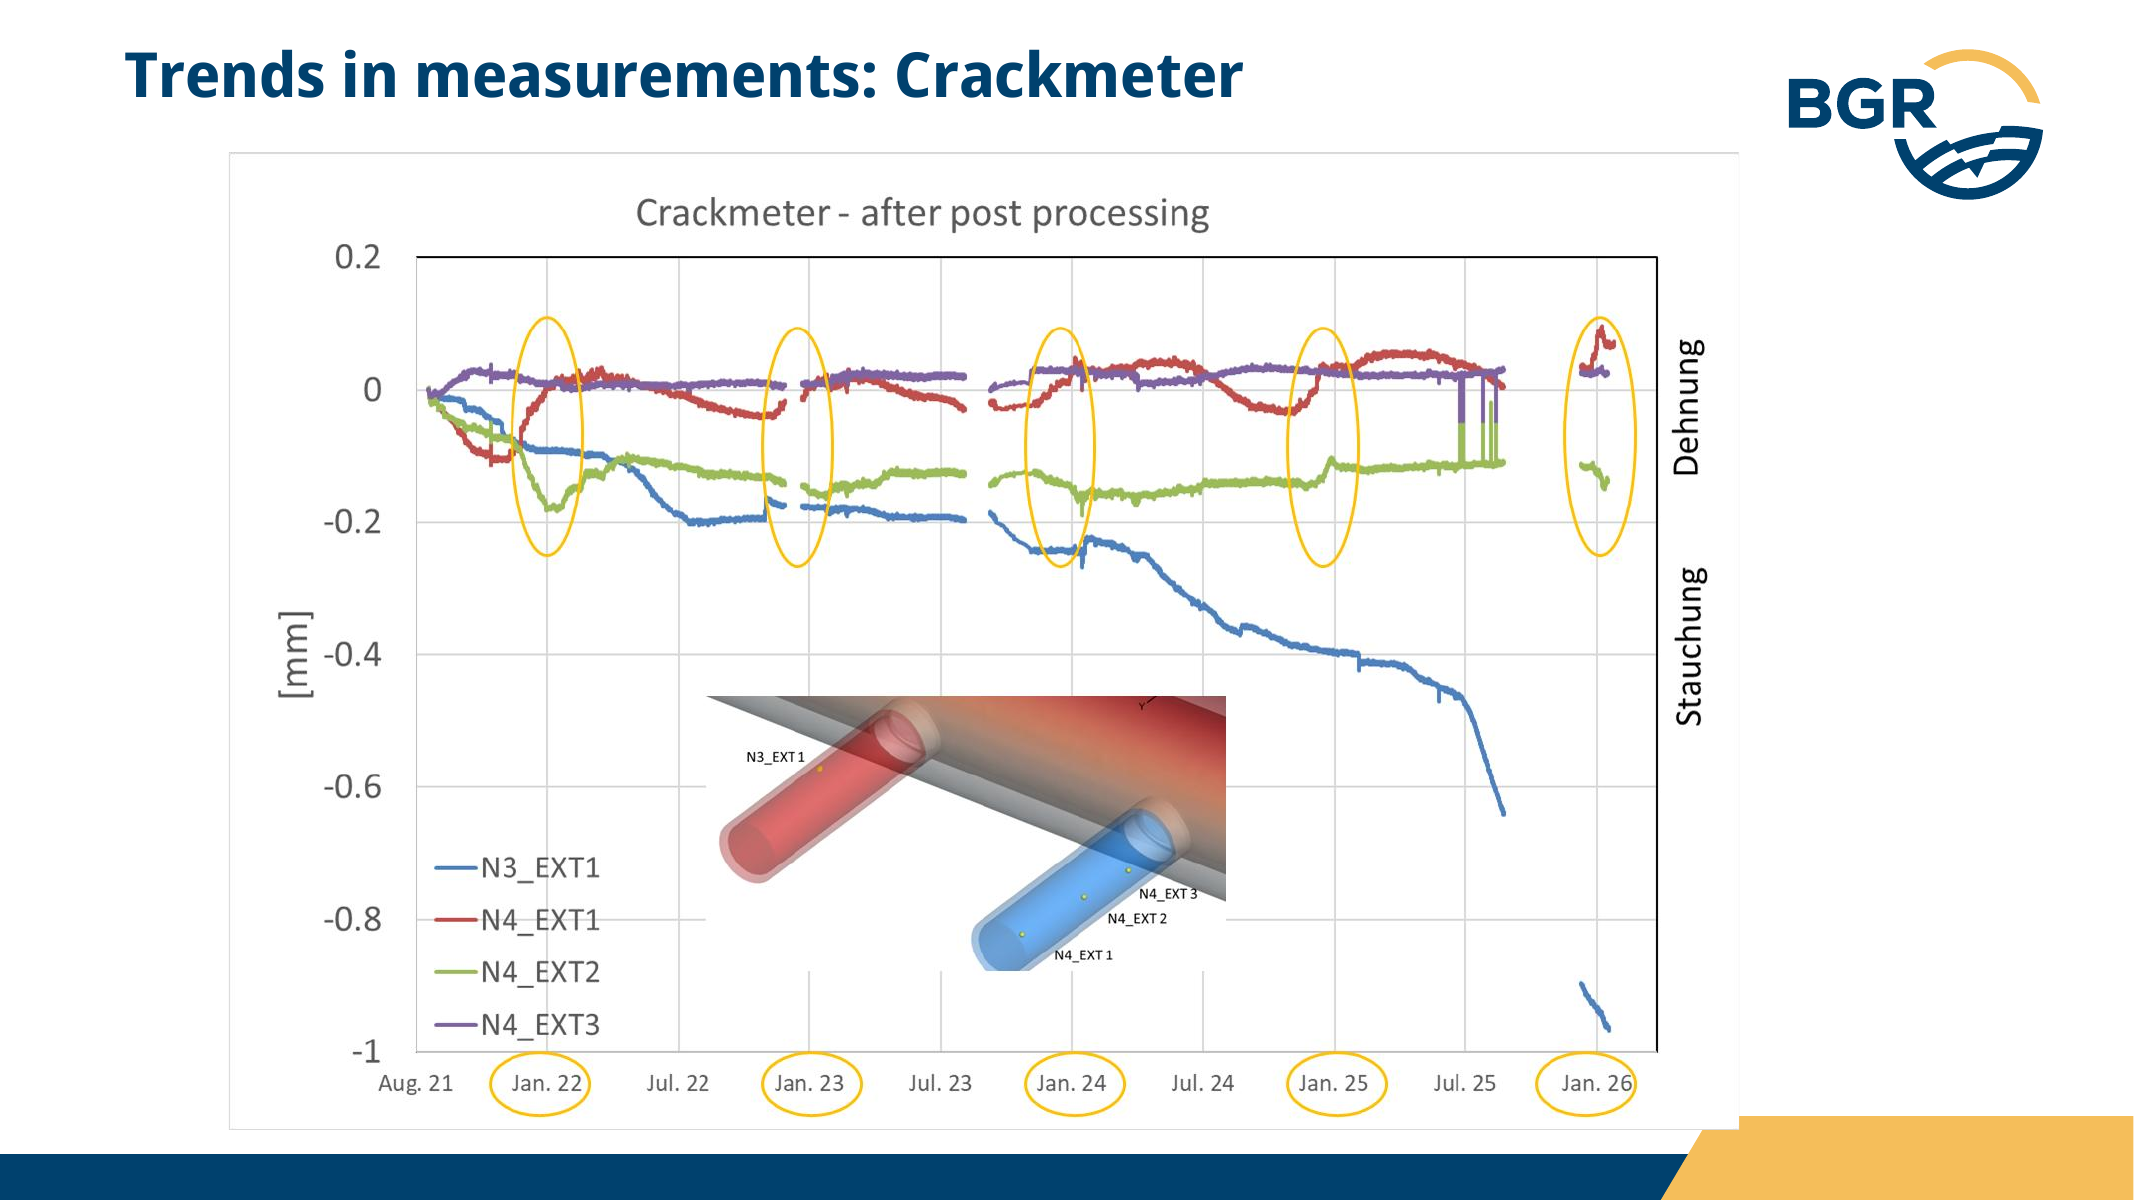
\includegraphics[width=0.92\textwidth]{resources/figures/measurement_crackmeter_trends.png}
  \captionof{figure}{Crackmeter trend evidence from the 2026 technical discussion slides.
  The plotted post-processed deformation is in millimetres and spans roughly August
  2021 to January 2026.  The slide shows seasonal markers and an instrument
  inset.  It is useful trend evidence, but not a residual-ready export because the
  paper still lacks positions, zero/reference convention, sign convention,
  uncertainty, and quality flags.}
  \label{fig:crackmeter-trends}
\end{center}

\paragraph{Uncertainty and reliability.}
The HM streams remain mostly blocked for hard residuals.  The source
scan found layout geometry, laser surface geometry, levelling slide rows, and
report/minute evidence, but no residual-ready Geoscope time series, laser
statistical product, or full levelling survey table
\citep[provided HM source files and generated trend figures]{CDAProvidedMeasurementFiles2025}.
A hard residual requires timestamps or survey epochs, values, units, support
geometry, reference-zero conventions, sign conventions, calibration, quality flags,
failure flags, and uncertainty or covariance.  The levelling slide gives a
detectable displacement of \(0.1\)--\(0.2\,\mathrm{mm}\) at 95\% confidence.  Across
the slide-summary points the largest settlement is CDA-O1
\((-2.1\,\mathrm{mm})\) and the largest uplift is the closed-twin point CDA-C4
\((+1.3\,\mathrm{mm})\).  Because only the open-twin values belong to the current
open-niche comparison and the slide still lacks the full survey table and
reference-frame metadata, these numbers remain qualitative validation context
rather than weighted residuals \citep[PDF pp.~5--6]{Levelling2026Email}.

\subsubsection*{Current computational use.}
\revadd{5}{Crackmeter and comparable HM streams are not active likelihood terms in
the present report.  They should be retained as qualitative validation, structural
priors, or future residual packages until numeric exports, reference zeros,
instrument axes, sign conventions, supports, and uncertainties are supplied.}{\annCommentFive}
With the available source data now, niche-surface cracks and other HM streams should
mostly be validation gates, qualitative priors, or future residual packages.  The
crackmeter source plot can test whether a model candidate gives plausible opening
or closure trends only after the measured component, zero date, sign convention,
instrument axis, and support are known.  Extensometers, convergence, miniprisma,
levelling, and laser scans have clear OGS displacement ties, but the current
workflow keeps mechanical parameters and prestress fixed.  Therefore these streams
should first reject mechanically implausible hydraulic candidates, support
EDZ/fracture scenarios, or define quality/disturbance flags; they should not yet
drive a coupled HM calibration
\citep[Table~1]{Ziefle2024Characterization}
\citep[abstract and Sec.~2]{Ziefle2017SeasonalHM}
\citep[PDF p.~4 and p.~8]{CDATDMinutes2026Email}
\citep[provided HM source files and generated trend figures]{CDAProvidedMeasurementFiles2025}.

If numeric exports are supplied, the operators are standard but stream-specific:
extensometers use projected displacement or strain along an instrument axis;
convergence uses point-pair displacement; crackmeters use relative displacement or
crack opening; levelling uses vertical displacement; laser scans use registered
surface differences with masks and registration covariance.  Auxiliary climate,
door, temperature, evapometer, or Geoscope context should enter as boundary
provenance, quality flags, or disturbance filters rather than interior residuals.

\subsubsection*{Grounding questions.}
\revnote{60}{\pdfAnnComment{43}{nemam predstavu, jak tahla data pouzit}{The HM
section answers with stream-specific future operators and keeps current use as
validation gates, qualitative priors, or future residual packages until numeric
exports and support conventions are supplied.}}
\gqGroundingTable{tab:grounding-other-hm}
{Grounding questions for Geoscope, crackometer, and other HM monitoring.}
{
\gqPair{gqGate}{Gate}{\qid{Q080} What does each HM stream measure?}{Extensometers measure axial deformation, crackmeters measure crack opening or
relative displacement, levelling measures vertical displacement, laser scans
measure surface differences, and auxiliary streams describe boundary or quality
context; each source export must confirm the exact quantity.}
\gqPair{gqGate}{Gate}{\qid{Q081} How should crackmeters link to OGS?}{Compare to relative displacement \((\uu_a-\uu_b)\cdot\nn\), where \(\nn\) is the
local crack-normal or instrument-axis direction, near-crack strain, or a
crack-aperture diagnostic only after the component and sign convention are known.}
\gqPair{gqPolicy}{Policy}{\qid{Q082} Can visible cracks justify permeability changes?}{Yes as an EDZ/fracture prior or scenario, but not as a weighted residual unless a
measured aperture or displacement operator is supplied.}
\gqPair{gqDiagnostic}{Diagnostic}{\qid{Q083} How should levelling, extensometers, and laser scans be used now?}{As diagnostic HM validation or rejection checks for candidate permeability and
boundary scenarios, because mechanical-parameter fitting is not currently grounded
as a model component.}
\gqPair{gqPolicy}{Policy}{\qid{Q084} Which other measurements can enter the OGS workflow?}{Any exported pressure, displacement, strain, crack-width, laser, climate,
temperature, evapometer, geology, or support-geometry stream can enter as an input,
residual, prior, mask, quality filter, or caveat once its support, time, units, and
uncertainty are explicit.}
\gqPair{gqBlocked}{Blocked}{\qid{Q085} What would fully ground HM residuals?}{Machine-readable values with timestamps or survey epochs, coordinates/supports,
units, reference-zero and sign conventions, instrument axes, failure/quality flags,
uncertainty or covariance, and a 3D-to-2D comparison policy.}
}
